\chapter{Inginerie software}

\section{Arhitectura aplicației}
Am ales să folosesc arhitectura MERN (MongoDB, Express.js, React, Node.js) la care am mai adăugat
două servere de Flask pentru recunoașterea vorbirii și clasificarea videoclip-urilor, o bază de
date Elasticsearch pentru căutare și Kibana pentru vizualizarea datelor din Elasticsearch.
\par
În figura de mai jos \ref{fig:project-architecture} este prezentată arhitectura aplicației.

\begin{figure}[h]
    \centering
    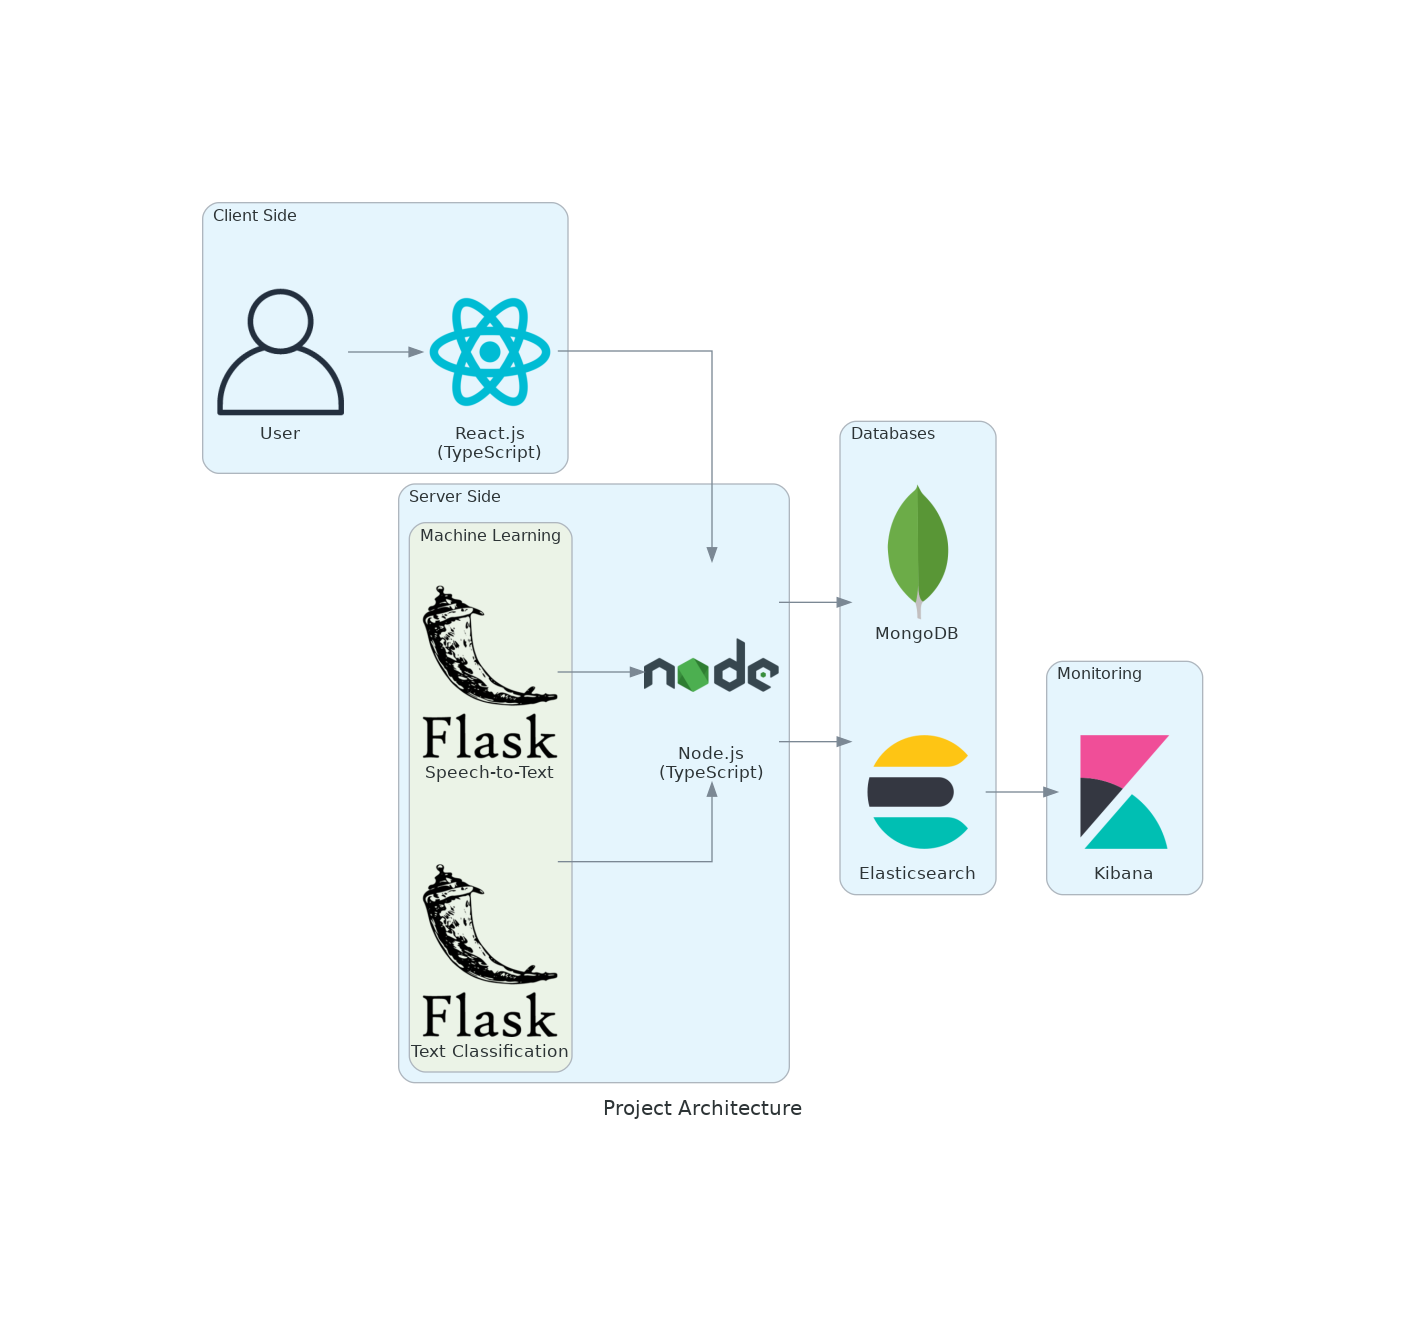
\includegraphics[width=0.6\textwidth]{project_architecture.png}
    \caption{Arhitectura aplicației}
    \label{fig:project-architecture}
\end{figure}


\section{Frontend}
Am folosit React și limbajul de programare TypeScript pentru interfața grafică a aplicației web. 
\par
React este o librărie JavaScript care simplifică procesul de dezvoltare a aplicațiilor web prin 
caracteristici specifice precum reutilizarea componentelor și actualizarea independentă a
elementelor interfeței grafice. TypeScript este un limbaj de programare creat de Microsoft care
extinde limbajului JavaScript cu tipuri statice, aspect util care îmbunătățește calitatea codului.

\subsection{React}
Librăria React impune o serie de concepte și bune practici care abstractizează și modularizează
codul aplicației web. Dintre acestea, cele mai importante sunt:

\begin{itemize}
    \item \textbf{Components}: Ideea de bază librăriei React o reprezintă componentele, elemente
    reutilizabile care încapsulează și izolează logica codului.
    \item \textbf{Props}: Proprietățile sunt parametrii transmiși de la componenta părinte
    la componenta copil, fiind folosite pentru customizarea comportamentului componentelor.
    \item \textbf{State}: Starea reprezintă datele interne ale componentelor, fiind folosite pentru
    actualizarea interfeței grafice din JSX.
    \item \textbf{Hooks}: Hooks sunt funcții speciale care permit interacțiunea cu starea și ciclul
    de viață al componentelor, fiind succesorul claselor din versiunile mai vechi ale librăriei.
    \item \textbf{Contexts}: Contextele sunt o modalitate de a controla transmiterea datelor între
    componente fără a folosi proprietăți, intuitiv, creând un fel de scope pentru componentele din
    interiorul contextului.
    \item \textbf{Models}: Deoarece folosim TypeScript, avem nevoie de modele pentru a defini tipurile
    de date folosite în aplicație.
    \item \textbf{Views/Pages}: Pot fi considerate componente principale, fiind rutele aplicației web.
    \item \textbf{Services}: Serviciile sunt funcții asincrone care primesc date din frontend,
    creează cereri HTTP către server (folosind \textit{Axios} sau \textit{Fetch}) și returnează
    răspunsurile primite de la server.
    \item \textbf{Utils}: Funcții utilitare care nu sunt legate de o componentă anume.
\end{itemize}

\subsection{Autentificare}
Autentificarea utilizatorilor nu folosește niciun serviciu extern, ci se bazează pe un sistem
propriu de înregistrare și logare. Fiecărei cereri de la client i se atașează un token JWT
(JSON Web Token) generat de server la logare/înregistrare, fiind folosit pentru a verifica
identitatea utilizatorului. 

\subsubsection{JWT}
JSON Web Token (JWT) encodează în structura sa 3 componente: header, payload și signature.
Header-ul stochează tipul de token și algoritmul de criptare, payload-ul conține informații
despre utilizator precum numele și data emiterii, iar signature-ul este un hash al primelor
două componente la care se mai adaugă un secret.

% poate adaugi o figura aici cu un exemplu de JWT, cea de jos e cam urata
% \begin{figure}[h]
%     \centering
%     \begin{minipage}{0.32\textwidth}
%         \begin{tcolorbox}[title=JWT Header, sharp corners]
%             \texttt{\{"alg": "HS256", "typ": "JWT"\}}
%         \end{tcolorbox}
%     \end{minipage}\hfill
%     \begin{minipage}{0.32\textwidth}
%         \begin{tcolorbox}[title=JWT Payload, sharp corners]
%             \texttt{\{"name": "Robert Trifan", "iat": 1516239022\}}
%         \end{tcolorbox}
%     \end{minipage}\hfill
%     \begin{minipage}{0.32\textwidth}
%         \begin{tcolorbox}[title=JWT Signature, sharp corners]
%             \texttt{HMACSHA256(base64UrlEncode(header) + "." + base64UrlEncode(payload))}
%         \end{tcolorbox}
%     \end{minipage}
% \end{figure}


\subsubsection{Înregistrare și logare}
Atât înregistrarea \ref{fig:register} cât și logarea \ref{fig:login} sunt realizate prin
intermediul unor formulare care cer informații precum numele, prenumele, adresa de email,
un nume de utilizator, o parolă și poză de profil. Pentru aceste formulare au fost folosite
validatoare care verifică dacă datele introduse sunt corecte.
\par
Odată ce datele sunt introduse, sunt validate încă o dată la nivel de server pentru a evita 
eventualele atacuri și, dacă sunt corecte, se generează un token JWT care este trimis înapoi
la client. Acest token este salvat în memoria locală a browser-ului, dar și în contextul
utilizatorului pentru a fi folosit în cererile ulterioare către server.
\par
Pentru deconectare, token-ul este șters din memoria locală și contextul utilizatorului.

\begin{figure}[h] 
    \centering
    \begin{minipage}{0.49\textwidth}
        \centering
        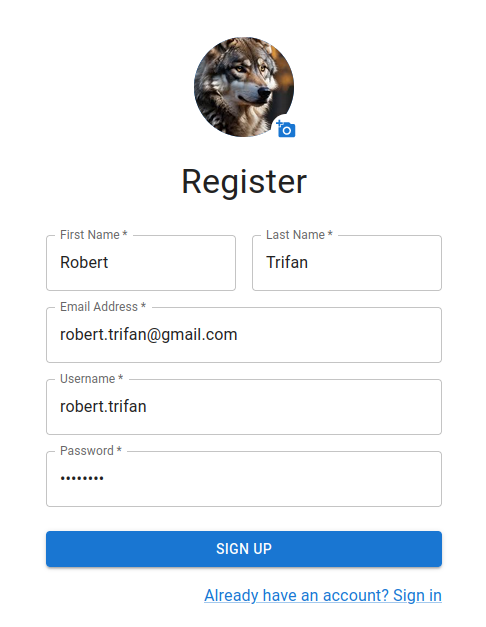
\includegraphics[width=0.9\textwidth]{register.png}
        \caption{Pagina de înregistrare}
        \label{fig:register}
    \end{minipage}\hfill
    \begin{minipage}{0.49\textwidth}
        \centering
        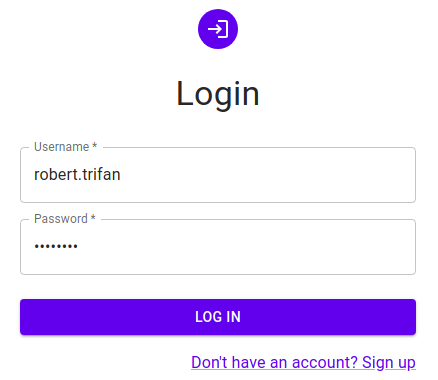
\includegraphics[width=0.9\textwidth]{login.png}
        \caption{Pagina de logare}
        \label{fig:login}
    \end{minipage}
\end{figure}

\subsubsection{Profil}
Pagina de profil prezină informați despre utilizator precum numele, prenumele, numele de utilizator,
adresa de email și poză de profil și îi permite acestuia să le actualizeze cu ajutorul unui formular.

\begin{figure}[h!]
    \centering
    \begin{minipage}{0.49\textwidth}
        \centering
        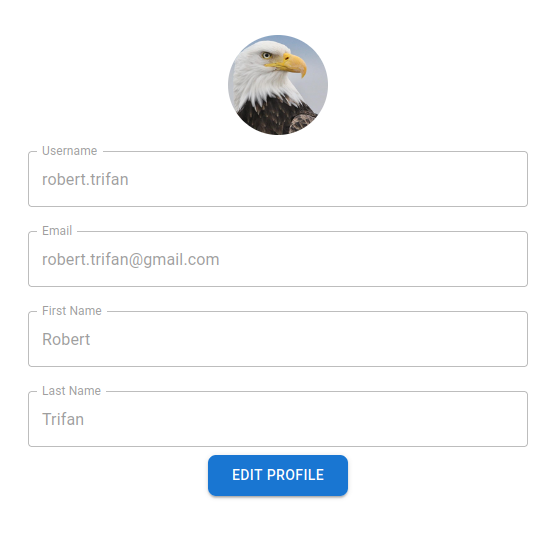
\includegraphics[width=0.9\textwidth]{profile.png}
        \caption{Pagina de profil}
        \label{fig:profile}
    \end{minipage}\hfill
    \begin{minipage}{0.49\textwidth}
        \centering
        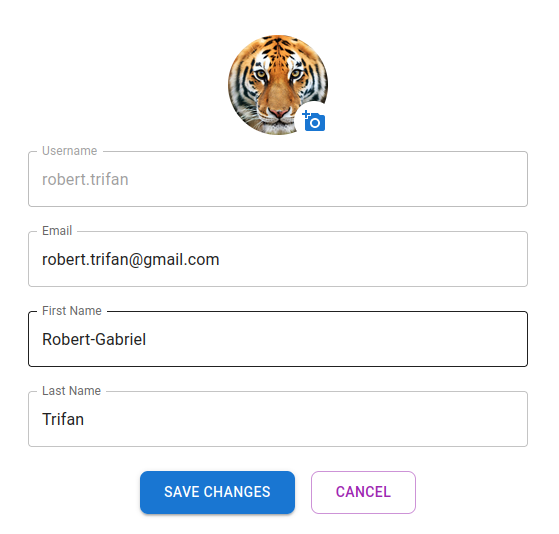
\includegraphics[width=0.9\textwidth]{profile-edit.png}
        \caption{Editare profil}
        \label{fig:profile-edit}
    \end{minipage}
\end{figure}

\vspace{1em}

\subsection{Video}
Platforma permite utilizatorilor să încarce videoclip-uri, să le vizualizeze și să
interacționeze cu acestea prin intermediul unor funcții precum aprecieri și comentarii.
\subsubsection{Încărcare videoclip}
Încărcarea videoclip-urilor se face print-un buton care redirecționează utilizatorul către
pagina de încărcare. Aici, utilizatorul poate selecta un fișier video și adăuga un titlu și
o descriere. După ce videoclip-ul este încărcat, acesta este trimis către server pentru a fi
prelucrat (stocarea în baza de date, extragerea subtitrărilor, clasificarea videoclip-ului).

\begin{figure}[h]
    \centering
    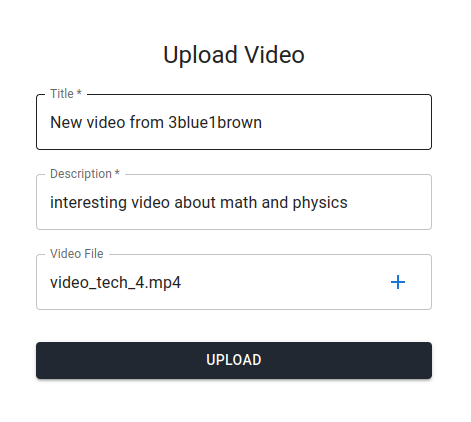
\includegraphics[width=0.5\textwidth]{upload.png}
    \caption{Pagina de încărcare a videoclip-urilor}
    \label{fig:upload}
\end{figure}

\subsubsection{Vizualizare}
Videoclip-urile încărcate sunt afișate pe pagina principală a aplicației web sub forma unui
grid, fiecare videoclip având un thumbnail, un titlu și numele autorului. Atunci când este 
accesat un videoclip, utilizatorul este redirecționat către o pagină dedicată unde poate
vizualiza videoclip-ul și interacționa cu acesta prin intermediul apreriilor și comentariilor.

\begin{figure}[h] 
    \centering
    \begin{minipage}{0.49\textwidth}
        \centering
        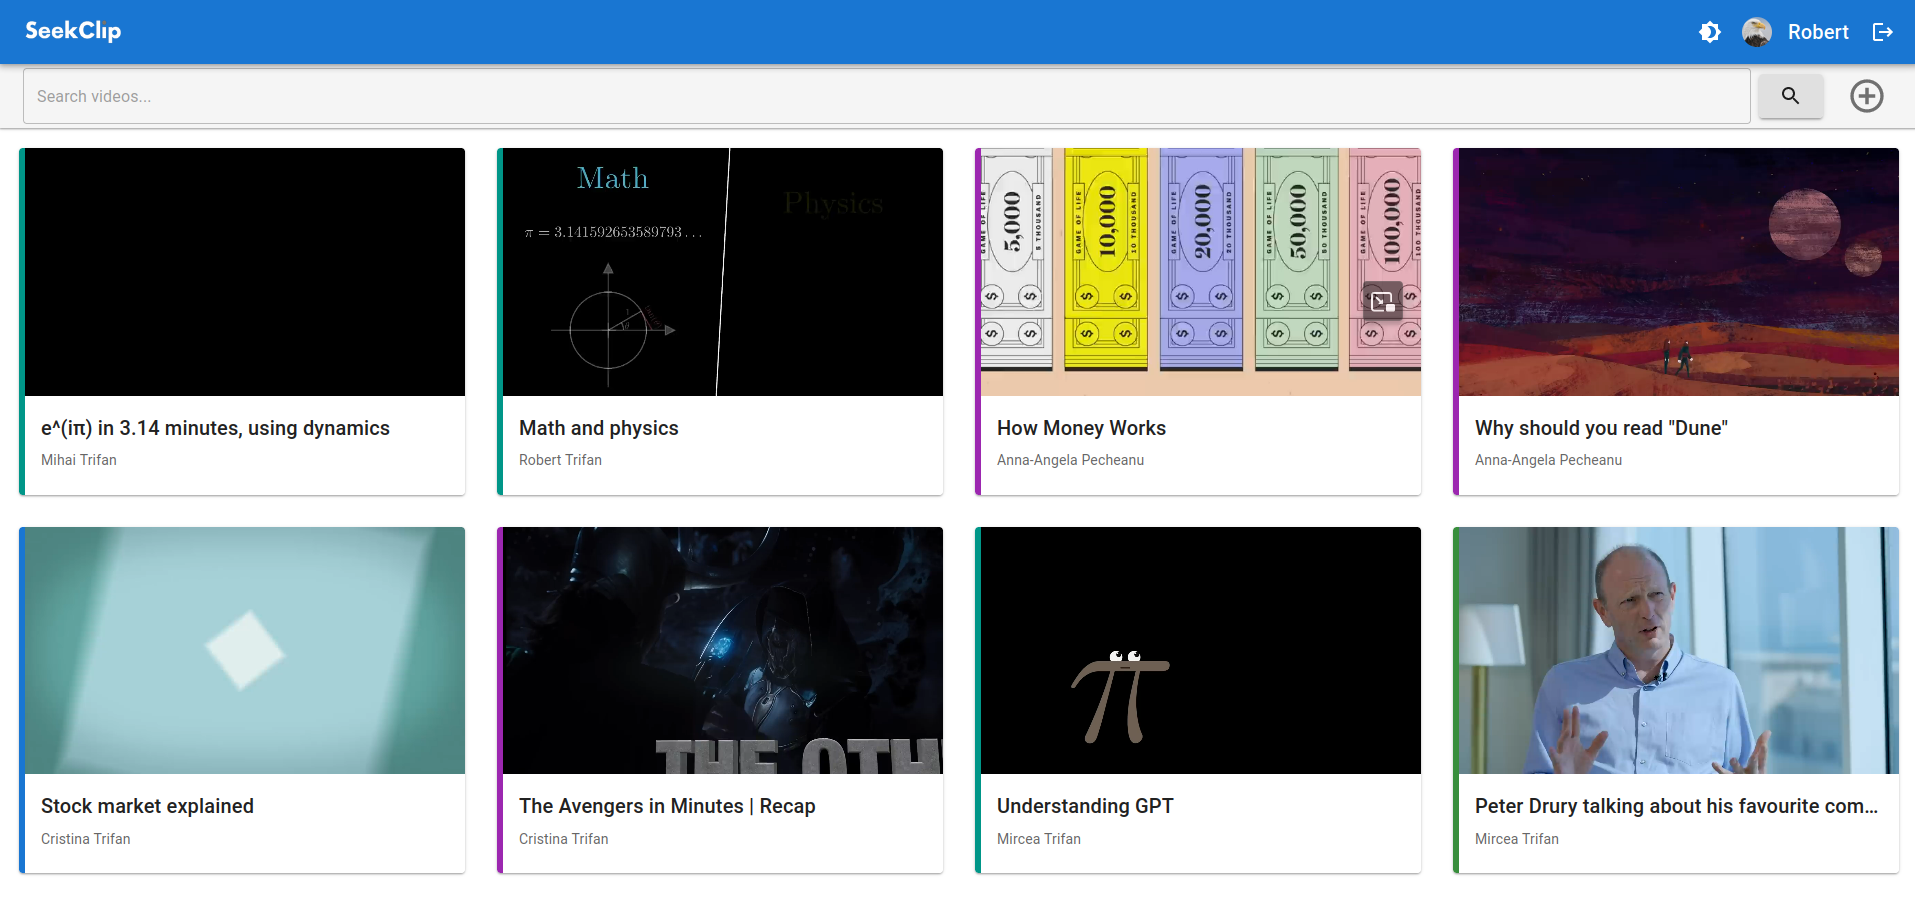
\includegraphics[width=0.9\textwidth]{video-grid.png}
        \caption{Grid de videoclip-uri}
        \label{fig:video-grid}
    \end{minipage}\hfill
    \begin{minipage}{0.49\textwidth}
        \centering
        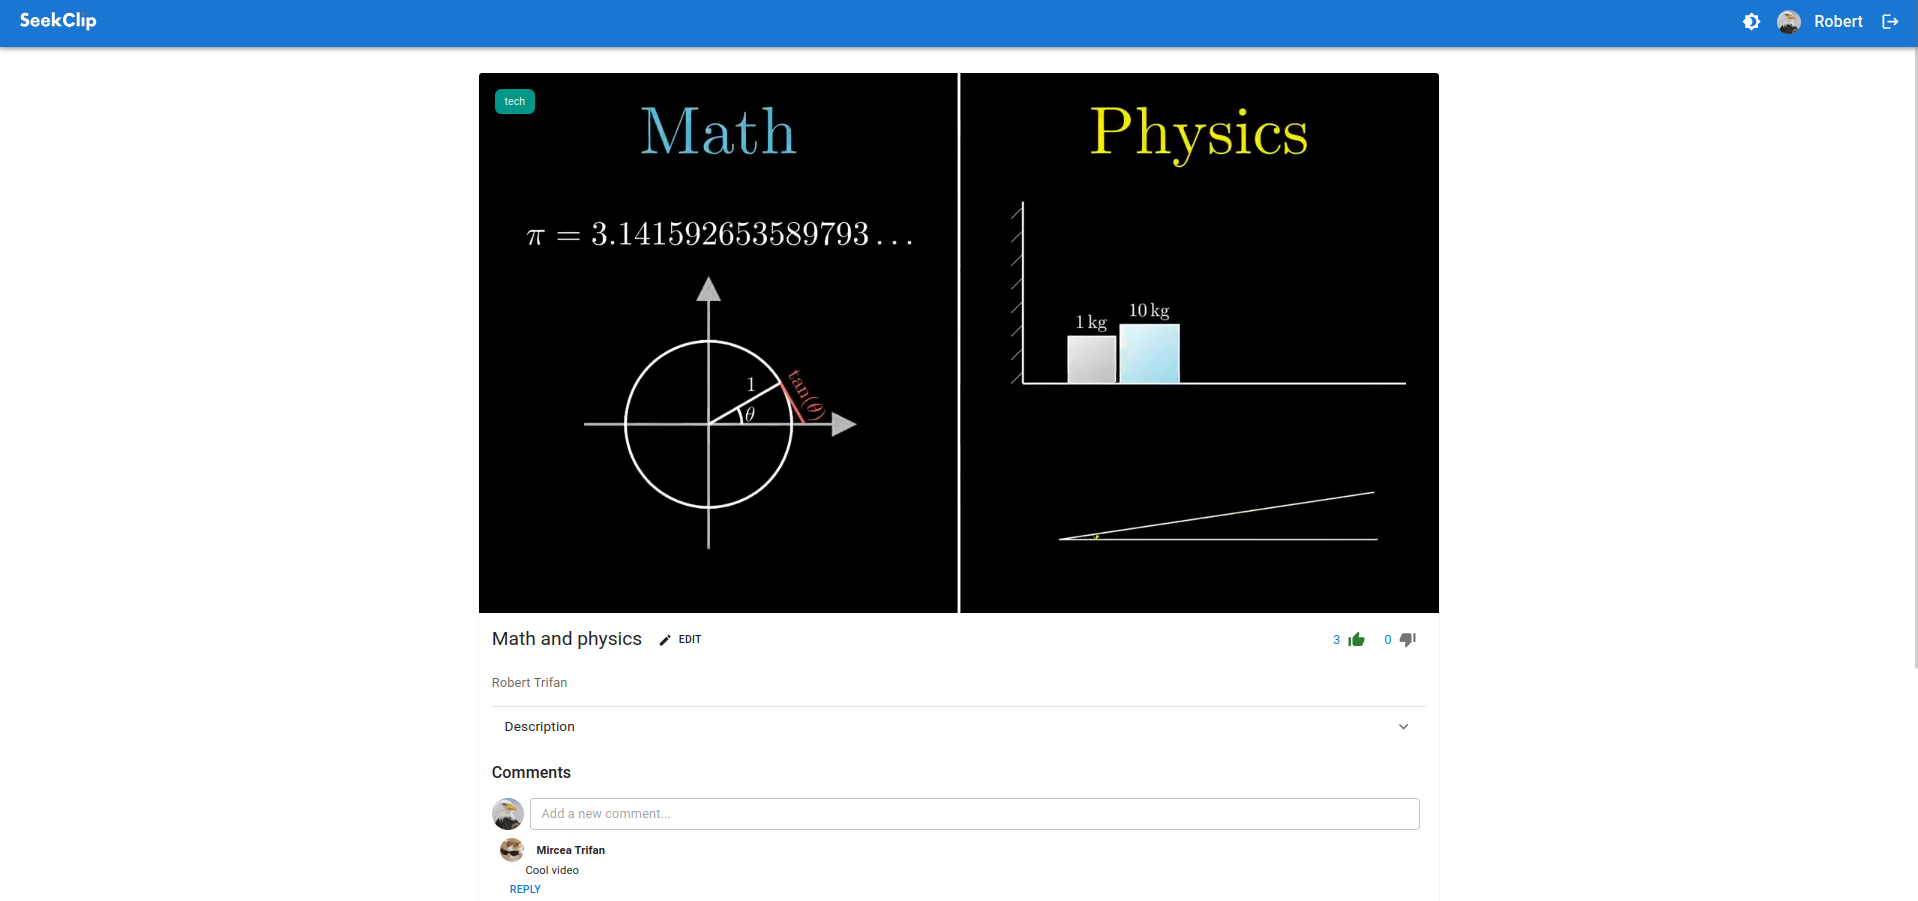
\includegraphics[width=0.9\textwidth]{video-view.png}
        \caption{Vizualizare videoclip}
        \label{fig:video-view}
    \end{minipage}
\end{figure}

\subsubsection{Editare}
Autorii videoclip-urilor încărcate pot accesa pagina de editare a videoclip-ului prin butonul
de editare de pe pagina de vizualizare. Fiind o rută protejată, utilizatorul trebuie să fie
autentificat și să fie autorul videoclip-ului pentru a putea schimba metadatele videoclip-ului.

\begin{figure}[h]
    \centering
    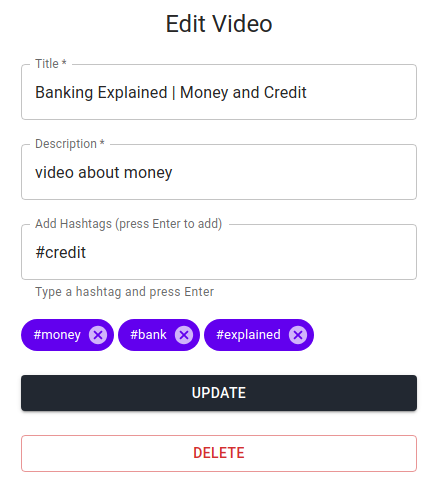
\includegraphics[width=0.6\textwidth]{video-edit.png}
    \caption{Editare videoclip}
    \label{fig:video-edit}
\end{figure}

\subsubsection{Aprecieri \& Comentarii}
Pagina de vizualizare a videoclip-ului permite utilizatorului să dea like, dislike videoclip-ului
sau să își retragă aprecierea și să adauge comentarii. 
\par
Fiecare videoclip reține o listă cu id-urile utilizatorilor care au dat like sau dislike și o
listă cu comentariile adăugate. De asemenea, utilizatorii pot răspunde la comentarii, creând astfel
o ierarhie de comentarii și pot edita sau șterge comentariile proprii.
\par
Dacă un comentariu are răspunsuri, atunci textul devine [deleted] fiind un \textit{soft-delete}.
Altfel, dacă un comentariu nu are răspunsuri, atunci acesta este șters complet din baza de date
fiind considerat un \textit{hard-delete}. Comentariile sunt sortate după data adăugării, cele mai
recente fiind afișate mai sus. 

\begin{figure}[h]
    \centering
    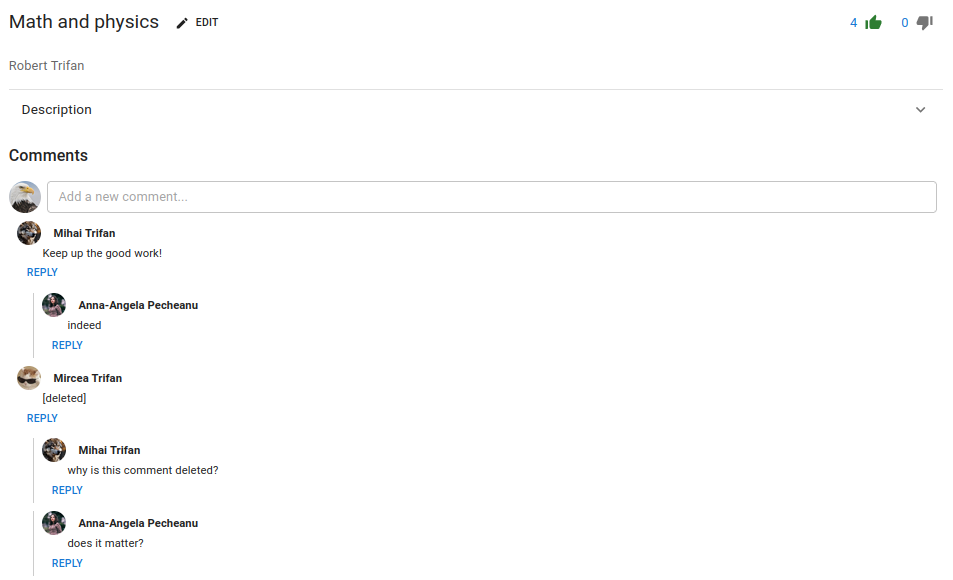
\includegraphics[width=0.95\textwidth]{video-interaction.png}
    \caption{Interacțiunea cu videoclip-ul}
    \label{fig:video-interaction}

\end{figure}

\par

Trebuie să menționez un detaliu important legat de ierarhia comentariilor. Ar fi foarte costisitor,
din punct de vedere al performanței, ca de fiecare dată când se șterge un comentariu să se reconstruiască
arborele de comentarii. De aceea, am creat un serviciu care rulează o dată pe zi, construieste ierarhia
comentariilor și șterge acele drumuri în arbore care nu mai sunt folosite. Mai multe detalii despre
acest serviciu se găsesc în secțiunea \ref{sec:cron-jobs}.

\subsection{Căutare}
\subsubsection{Bara de căutare}
Pe pagina principală a aplicației web se află o bară de căutare care permite utilizatorului
introducerea unor cuvinte cheie specifice videoclip-urilor pe care le caută.
\ref {fig:search-bar}.

\vspace{1em}
\begin{figure}[h]
    \centering
    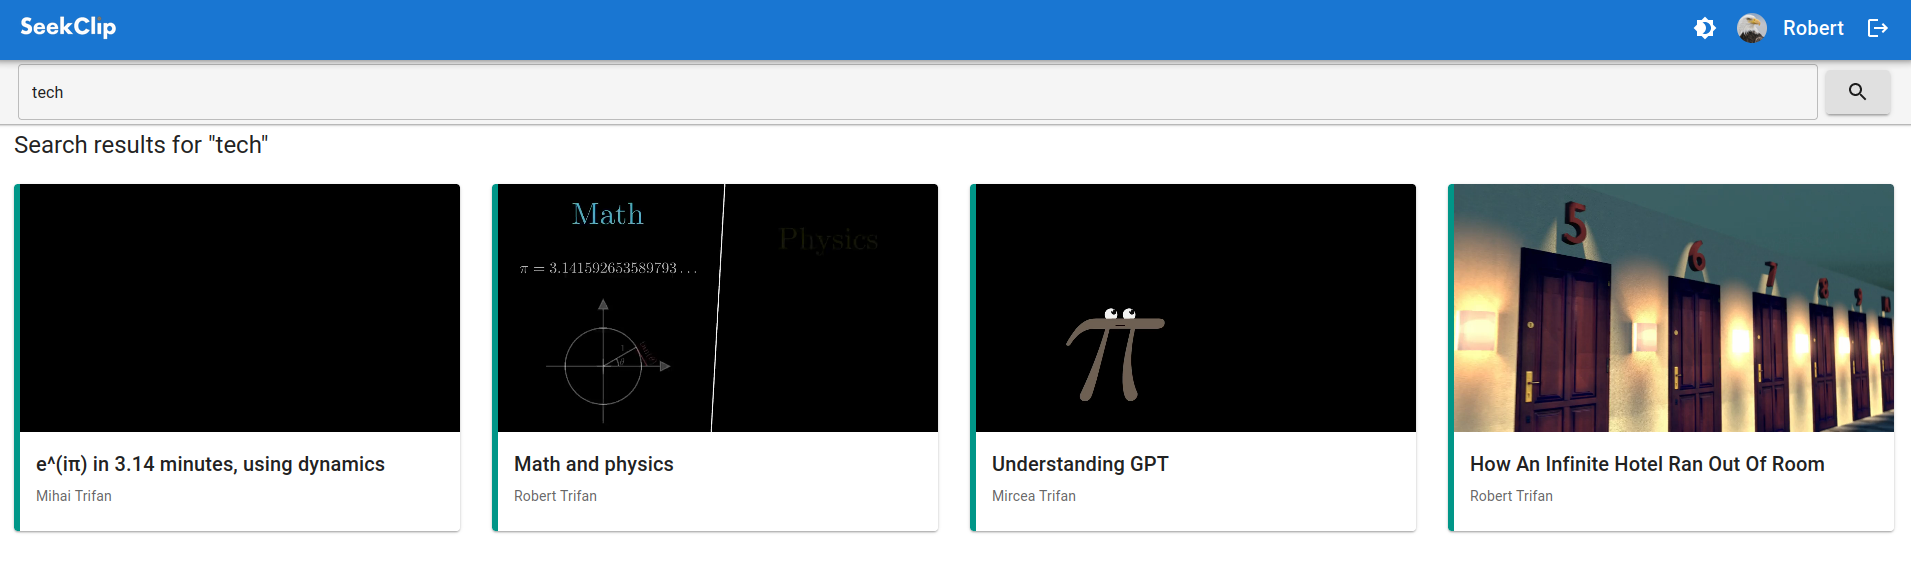
\includegraphics[width=0.95\textwidth]{search-bar.png}
    \caption{Bară de căutare}
    \label{fig:search-bar}
\end{figure}

\par
Când utilizatorul introduce textul în bara de căutare, aplicația web trimite o cerere 
către server care caută videoclip-urile într-o bază de date Elasticsearch. Rezultatele
sunt afișate pe aceeași pagină, sub forma unui grid asemănător cu cel de pe pagina principală.

\subsection{Temă}
Întreaga aplicație web poate fi personalizată prin intermediul a două teme: light și dark.
Utilizatorul poate schimba tema din navbar cu ajutorul unui buton care schimbă valoarea
unei variabile din contextul temei și propagă această schimbare în întreaga aplicație web.

\begin{figure}[h]
    \centering
    \begin{minipage}{0.49\textwidth}
        \centering
        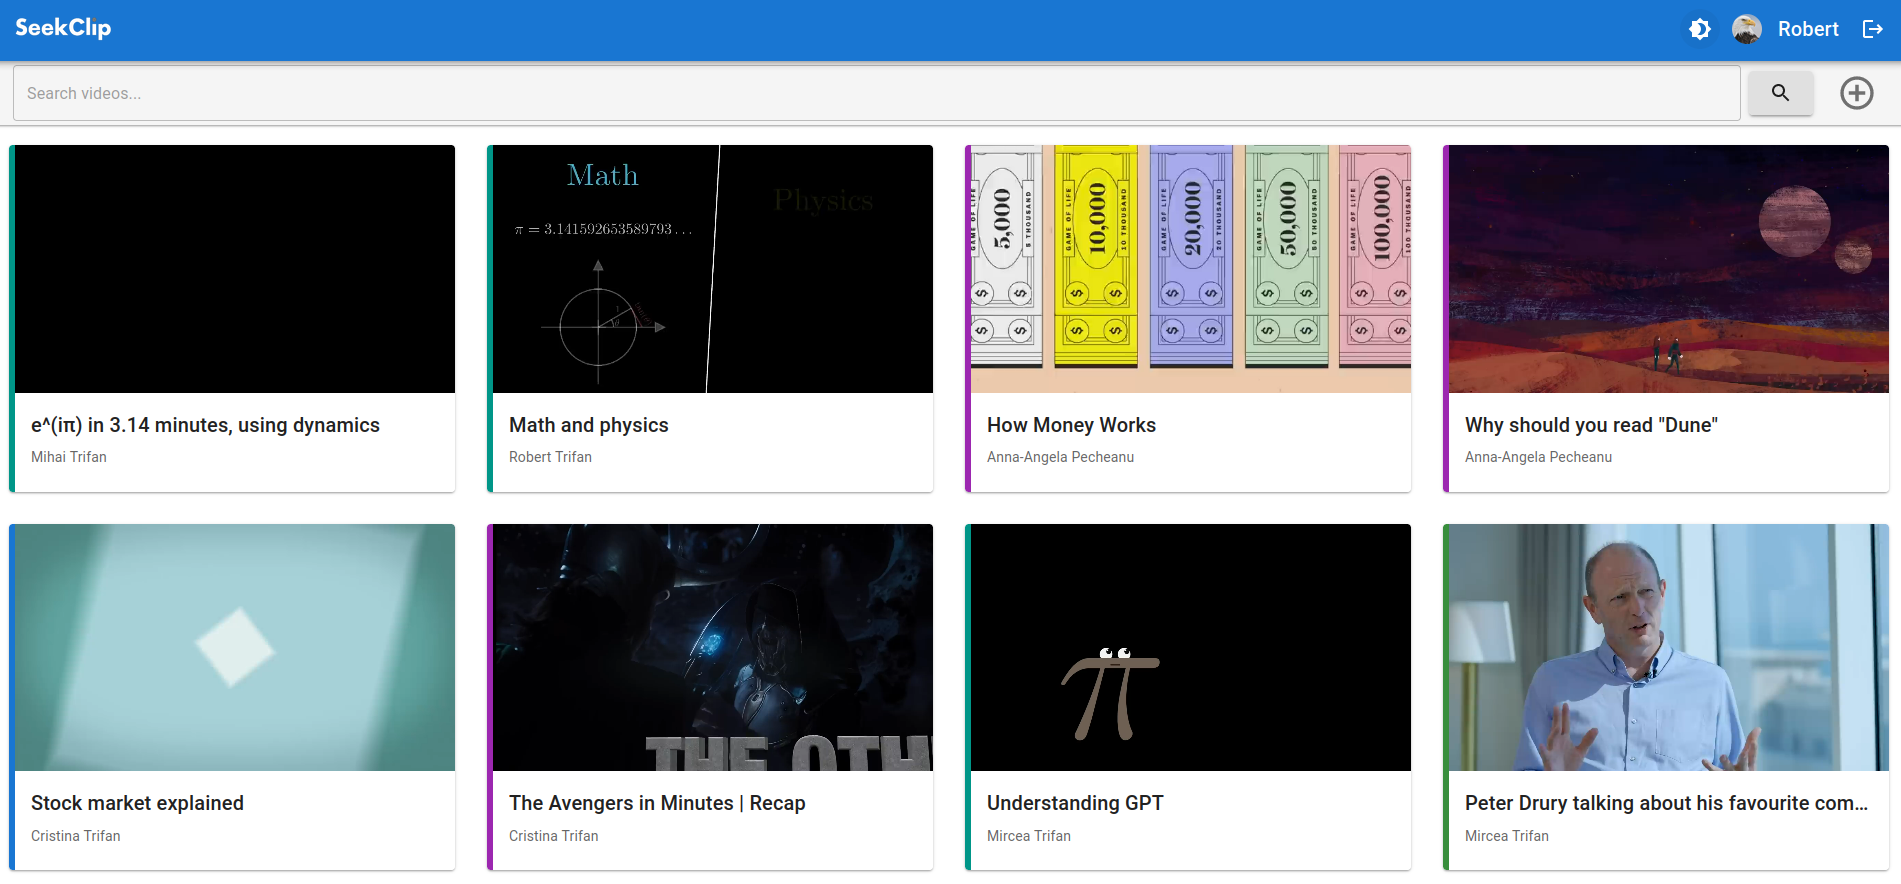
\includegraphics[width=0.9\textwidth]{light-theme.png}
        \caption{Tema light}
        \label{fig:light-theme}
    \end{minipage}\hfill
    \begin{minipage}{0.49\textwidth}
        \centering
        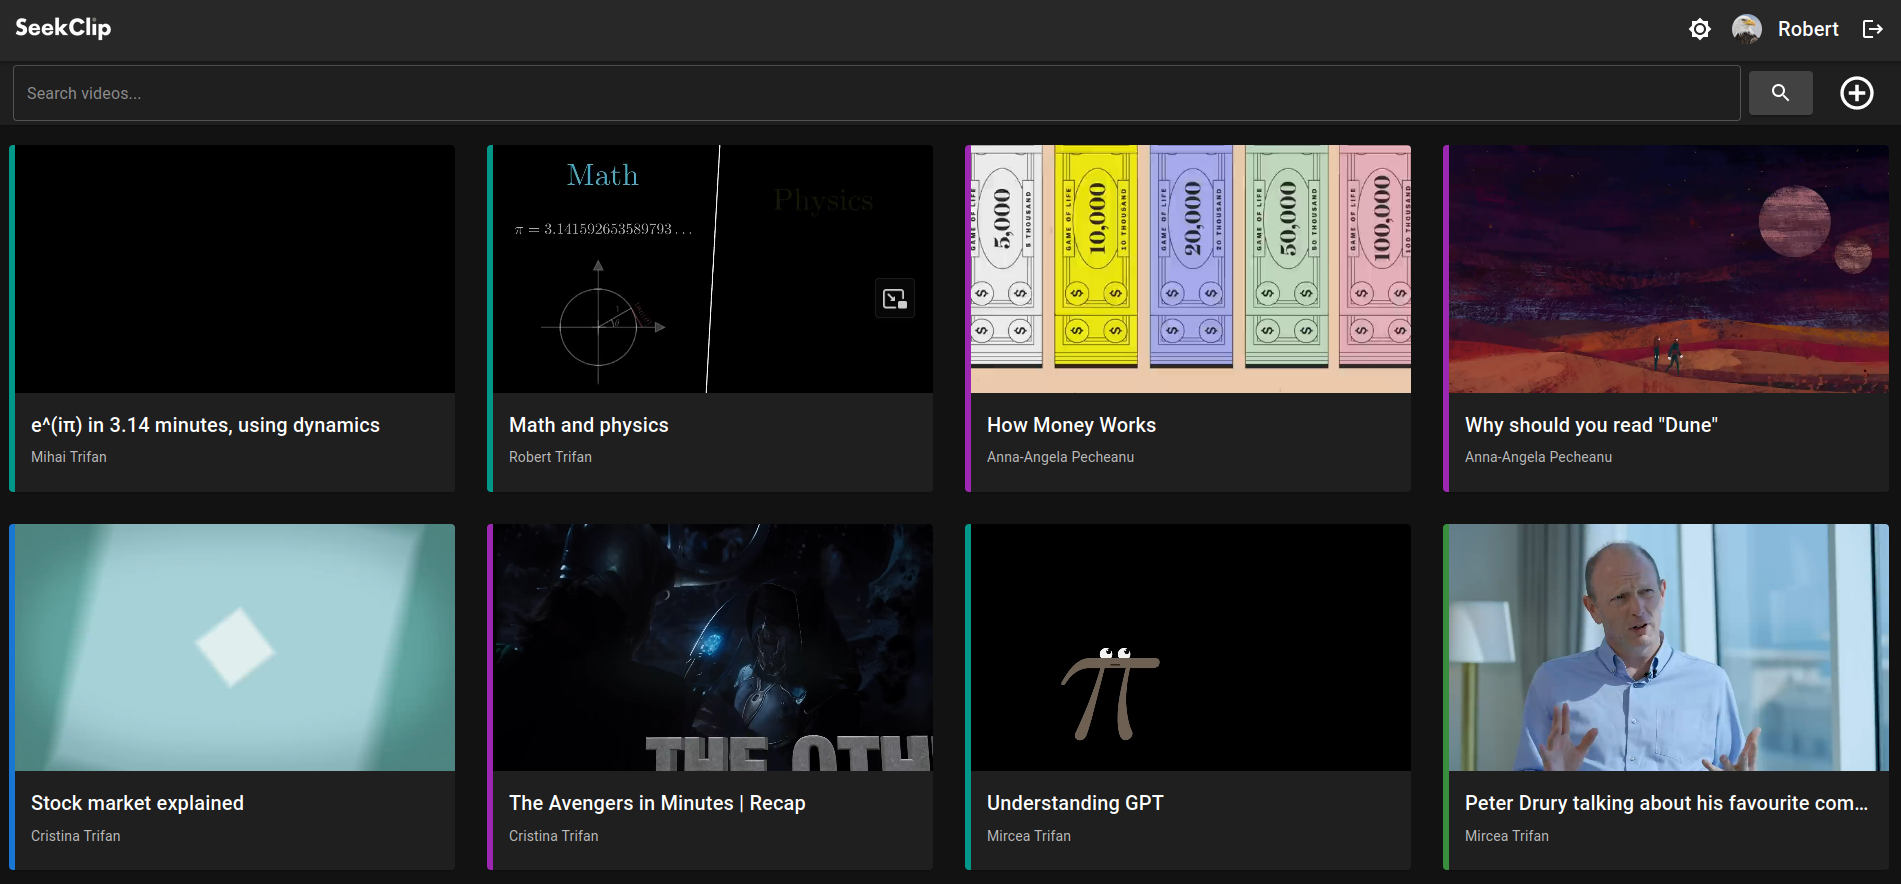
\includegraphics[width=0.9\textwidth]{dark-theme.png}
        \caption{Tema dark}
        \label{fig:dark-theme}
    \end{minipage}
\end{figure}

\subsection{Rute protejate}
Pentru a interzice accesul la anumite pagini din motive de securitate, am folosit un sistem
de rute protejate:
\begin{itemize}
    \item \textbf{User Protected}: se asigură că sunt accesate doar de utilizatori autentificați,
    în caz contrar fiind redirecționați către pagina de logare; de exemplu, pagina de profil,
    încărcarea videoclip-urilor, postarea de comentarii/aprecieri.
    \item \textbf{Video Owner Protected}: se asigură că sunt accesate doar de autorii videoclip-urilor,
    și implicit de utilizatorii autentificați, în caz contrar fiind redirecționați către pagina principală;
    de exemplu, editarea videoclip-urilor.
\end{itemize}

\section{Backend}

\subsection{Express Server - Procesarea cererilor}
Am creat un server Node.js folosind Express.js în limbajul de programare TypeScript care
gestionează cererile primite de la client și le rutează către serviciile corespunzătoare.
\par
Astfel, codul este structurat: 

\begin{itemize}
    \item \textbf{Routes}: definesc rutele serverului și asociază cererile primite cu funcțiile
    corespunzătoare din controlere.
    \item \textbf{Controllers}: conțin funcțiile care procesează cererile primite de la client
    și apelează serviciile necesare.
    \item \textbf{Middlewares}: funcții care se execută între primirea cererilor și procesarea
    acestora, adăugând/verificând informații suplimentare din cererea primită.
    \item \textbf{Models}: definește structura entităților folosite în baza de date MongoDB 
    și a interfețelor pentru a asigura tipurile de date.
    \item \textbf{Utils}: funcții utilitare care facilitează procesarea cererilor.
    \item \textbf{Config}: inițializează comunicarea cu alte servicii precum baza de date Elasticsearch.
\end{itemize}

\subsubsection{REST API}
Comunicarea între client și server se face prin intermediul unui REST API. Prin definiție,
REST (Representational State Transfer) impune existența a 3 componente: client, server și resurse.
\par
Clientul îl reprezintă aplicația web care face cereri către server, serverul este aplicația
care primește gestionează cererile și returnează răspunsuri, iar resursele sunt datele stocate
în baza de date pe care serverul le manipulează.

\par
Conceptul de REST API are la bază 6 principii:
\begin{itemize}
    \item \textbf{Separarea client-server}: clientul și serverul sunt entități separate și izolate,
    serverul nu poate face cereri către client, doar clientul poate face cereri către server; 
    în acest fel, cele două entități pot evolua independent.
    \item \textbf{Uniform Interface}: având în vedere diversitatea limbajelor de programare folosite
    atât pentru client cât și pentru server, este necesară o interfață comună, independentă de limbaj
    care să faciliteze comunicarea între cele două entități; astfel REST API este construit peste 
    protocolul HTTP și folosește metodele standardizate GET, POST, PUT, DELETE.
    \item \textbf{Stateless}: fiecare cerere primite de la client conține toate informațiile necesare
    pentru a fi procesată cu succes, serverul nefiind nevoit să păstreze informații despre cererile
    anterioare.
    \item \textbf{Layered System}: cererea primită de la client poate trece prin mai multe straturi
    intermediare folosite pentru a îmbunătăți performanța, securitatea sau scalabilitatea aplicației.
    \item \textbf{Cacheable}: cererile anterioare pot fi stocate în cache pentru a fi refolosite
    la cereri ulterioare, reducând astfel timpul de răspuns și traficul de date între client și server.
    \item \textbf{Code on Demand (Optional)}: serverul poate trimite cod executabil către client pentru
    a fi rulat în browser, însă această funcționalitate este opțională
\end{itemize}

\subsubsection{Codurile de stare HTTP}
Pentru a comunica rezultatul unei cereri, există un standard de coduri HTTP împărțit în
următoarele 5 categorii:
\begin{itemize}
    \item \textbf{1xx}: informații, cererea a fost primită, se continuă procesarea.
    \item \textbf{2xx}: succes, cererea a fost primită, procesată și răspunsul a fost generat cu succes.
    \item \textbf{3xx}: redirecționare, clientul trebuie să facă o altă cerere pentru a obține răspunsul.
    \item \textbf{4xx}: erori de la client, cererea a fost greșită sau nu poate fi procesată.
    \item \textbf{5xx}: erori de la server, serverul a întâmpinat o problemă în procesarea cererii.
\end{itemize}

\subsubsection{Routes}
Rutele sunt construite recursiv, plecând de la rădăcină și adăugând pentru fiecare API 
un nou nivel de rute. În cadrul aplicației noastre, am definit următoarele rute:

\begin{itemize}
    \item \textbf{/api/auth}: rutele responsabile de autentificarea utilizatorilor, care mai apoi 
    se specializează în /api/auth/register și /api/auth/login.
    \item \textbf{/api/user}: rutele responsabile de gestionarea informațiilor utilizatorilor, se 
    specializează în /api/user/:username și /api/user/update/:username.
    \item \textbf{/api/video}: rutele responsabile de gestionarea videoclip-urilor, se specializează
    în operațiile CRUD (Create, Read, Update, Delete) pentru videoclipuri și a interacțiunilor cu acestea.
    \item \textbf{/api/comment}: rutele responsabile de gestionarea comentariilor, aduc funcționalități
    precum adăugarea, editarea și ștergerea comentariilor.
\end{itemize}

\subsubsection{Middlewares}
Middleware-urile sunt funcții care se execută între primirea cererii și procesarea acesteia,
de obicei adăugând sau verificând informații suplimentare din cererea primită. În cadrul
aplicației noastre, am folosit două middleware-uri:

\begin{itemize}
    \item \textbf{Auth Middleware}: se adaugă la cererile care necesită ca utilizatorul să fie
    autentificat, verificând astfel existența token-ului JWT și dacă acesta este valid. Verificarea
    se face prin decriptarea token-ului și verificarea semnăturii cu ajutorul secretului stocat
    pe server. Fiecare cerere are în header-ul ei un câmp \textit{Bearer Token} care conține
    token-ul JWT. Odată decriptat, middleware-ul adaugă în corpul cererii informațiile despre
    utilizatorul autentificat.
    \item \textbf{Multer Middleware}: se folosește pentru cererile care necesită încărcarea unor
    fișiere de tip imagine sau videoclip; middleware-ul se asigură că fișierul are formatul corect
    (de exemplu, imaginea este de tip .jpg/.png/.jpeg și videoclip-ul este de tip .mp4/.mov/.avi).
    Acesta creează un director în interiorul căruia se salvează fișierul încărcat și adaugă
    calea către fișier în baza de date. Serverul expune apoi url-ul către id-ul fișierului
    încărcat pentru a putea fi accesat de client.
    
\end{itemize}

\subsubsection{Models}
Modelele sunt folosite pentru a defini structura entităților folosite în baza de date MongoDB. Deci,
pentru fiecare entitate din baza de date, definim o \textit{Schema} care conține câmpurile, tipurile
de date ale acestora, restricțiile și referințele către alte entități. În cadrul aplicației noastre,
am definit următoarele modele:
\begin{itemize}
    \item \textbf{User}: reține pentru fiecare utilizator numele, prenumele, adresa de email, numele
    de utilizator, parola și poza de profil. De asemenea, adaugă și restricții pentru a asigura
    unicitatea numelui de utilizator și a adresei de email, tipuri de date pentru fiecare câmp,
    necesitatea completării câmpurilor și lungimea minimă și maximă a câmpurilor.
    \item \textbf{Video}: reține pentru videoclip informații precum url-ul unde este stocat, titlul,
    descrierea, id-ul autorului, textul din videoclip și calea către subtitrări în formatul .vtt,
    o listă cu id-urile utilizatorilor care au dat like/dislike, topicul videoclip-ului și data.
    Restricțiile impuse sunt similare cu cele de la modelul User, au grijă ca fiecare videoclip să
    aibă obligatoriu metadatele necesare și să aibă un autor valid. De asemenea, sunt menționate
    și tipurile de date ale câmpurilor.
    \item \textbf{Comment}: reține pentru fiecare comentariu textul, id-ul autorului, id-ul videoclip-ului,
    dacă este șters sau nu (\textit{soft-delete/hard-delete}) pentru eficientizarea procesului de ștergere
    a comentariilor, și id-ul comentariului la care răspunde pentru a putea crea ierarhia comentariilor.
    Schema modelului impune restricția ca id-ul autorului și id-ul videoclip-ului să fie obligatorii,
    iar textul să fie completat.
\end{itemize}


\subsubsection{Controllers}
Fiecare rută menționată anterior are asociată un controller care procesează cererea primită, 
apelează serviciile necesare și returnează răspunsul.
\par
Menționez aici câteva dintre funcțiile mai importante:

\begin{itemize}
    \item \textbf{register/login}: funcții care se ocupă de înregistrarea și logarea utilizatorilor,
    creează token-ul JWT folosind secretul stocat pe server și id-ul utilizatorului, verifică
    existența utilizatorului în baza de date și returnează token-ul JWT.
    \item \textbf{getUserByUsername/updateUserProfile}: funcții folosite pentru a obține informații
    despre utilizator, respectiv pentru a actualiza informațiile utilizatorului. Se observă aici
    cum funcția de actualizare a profilului folosește atât middleware-ul de autentificare pentru a
    se asigura că doar utilizatorul autentificat poate actualiza profilul, cât și middleware-ul
    de încărcare a fișierelor pentru a actualiza poza de profil. Ambele funcții accesează baza de
    date pentru a obține sau actualiza informațiile și returnează răspunsul.
    \item \textbf{addComment/udpateComment/deleteComment/getCommentsForVideo}: după cum sugerează
    și numele, sunt funcții care permit adăugarea, actualizarea, ștergerea și obținerea comentariilor
    pentru un videoclip. Funcțiile de adăugare și actualizare a comentariilor folosesc middleware-ul
    de autentificare pentru a se asigura că doar utilizatorii autentificați pot executa aceste operații.
    Întâlnim aici si funcția \textit{populate} din Mongoose care ne permite să expandăm referințele
    din baza de date, în cazul nostru, să obținem informații despre autorul comentariului.
    \item \textbf{uploadVideo/updateVideo/deleteVideo}: funcții care permit încărcarea videoclip-urilor,
    actualizarea și ștergerea acestora. Fiecare funcție necesită middleware-ul de autentificare pentru
    a asocierea unui videoclip cu autorul său, iar funcțiile de actualizare și ștergere a videoclip-urilor
    permit doar autorului videoclip-ului să execute aceste operații. Serviciul de încărcare a video-urilor
    apelează la rândul lui cele două servere de Flask pentru extragerea subtitrărilor și clasificarea
    videoclip-ului.
    \item \textbf{getAllVideos/getVideosByUser/getVideoById}: funcții care permit accesarea videoclip-urilor
    din baza de date în diferite moduri: toate videoclip-urile, videoclip-urile unui utilizator sau un
    videoclip anume după id-ul său. Funcțiile caută la rândul lor în baza de date după criteriile
    specificate și returnează răspunsul.
    \item \textbf{likeVideo/dislikeVideo/getLikes/getDislikes}: funcții care permit interacțiunea cu 
    un videoclip, adăugând sau ștergând id-ul utilizatorului care a dat like/dislike din lista de
    referințe a videoclip-ului. De asemenea, sunt tratate aici și cazurile speciale în care utilizatorul
    dă dislike după ce a dat like sau invers și cazul în care utilizatorul retrage aprecierea.
    \item \textbf{searchVideos}: funcție care primește din cerere cuvintele cheie (titlu, descriere,
    subtitrări, topic), accesează baza de date Elasticsearch pentru a căuta videoclip-urile care conțin
    acele cuvinte și returnează o listă cu id-urile videoclip-urilor găsite. De menționat că am ales
    un threshold de 1.0 pentru a filtra rezultatele mai slabe și am setat parametrul \textit{fuzziness} 
    pe \textit{AUTO} pentru a permite căutări aproximative.

    
\end{itemize}

\subsubsection{Utils}
Funcțiile utilitare nu depind de o anumită entitate și sunt folosite pentru a facilita procesarea
cererilor. În cadrul aplicației noastre, am definit următoarele funcții utilitare:

\begin{itemize}
    \item \textbf{getTranscription}: înainte de a trimite cererea către serverul de Flask pentru 
    recunoașterea vorbirii, e nevoie să extragem întâi secvența audio din videoclip deoarece 
    modelul lucrează cu fișiere audio. Folosesc pentru acest lucru librăria \textit{ffmpeg-extract-audio}
    care permite procesarea fișierelor video și extragerea secvenței audio. De asemenea, secvența
    audio fiind destul de mare, creez un flux de date folosind \textit{fs.createReadStream} și 
    atașez acest flux la cererea către serverul de Flask.
    \item \textbf{getTopic}: după ce am obținut subtitrările videoclip-ului, folosesc un serviciu
    extern pentru a clasifica fiecare videoclip în funcție de metadatele sale și a subtitrărilor.
    Astfel, creez o cerere către serverul de Flask pentru clasificare și returnez topicul videoclip-ului.
\end{itemize}

\subsubsection{Config}
Configurările sunt folosite pentru a inițializa comunicarea cu alte servicii precum baza de date
Elasticsearch. Folosesc două fișiere de configurare: \textit{elasticsearchClient.ts} și
\textit{elasticsearchSetup.ts}. Primul creează un client Elasticsearch folosind librăria
\textit{@elastic/elasticsearch} și exportă clientul pentru a fi folosit în servicii, iar al doilea
creează un index specific Elasticsearch pentru a stoca informații necesare căutării videoclip-urilor.
Deoarece aplicația este un prototip, folosesc o singură replică pentru index și un singur shard.

\subsubsection{Expunerea datelor}
Datele multimedia precum: videoclip-urile, subtitrările și pozele de profil sunt stocate 
pe mașina serverului, în directoare separate: \textit{/uploads}, \textit{/captions} și
\textit{/profile-pictures}. Aceste directoare sunt expuse către client folosind
\textit{express.static} și pot fi accesate la link-ul unde rulează serverul concatenat
cu numele fișierului stocat în baza de date.


\begin{verbatim}
    app.use('/uploads', express.static('uploads'));
    app.use('/captions', express.static('captions'));
    app.use('/profile-pictures', express.static('profile-pictures'));
\end{verbatim}

\subsubsection{Criptarea parolelor}
Serverul folosește algoritmul de criptare \textit{bcrypt} pentru a stoca parolele utilizatorilor
în baza de date. Algortimul de criptare are la bază următoarele concepte:

\begin{itemize}
    \item \textbf{Salting}: librăria \textit{bcrypt} generează automat un salt (o valoare aleatoare)
    pentru fiecare parolă, pentru a preveni atacurile de tip \textit{rainbow table}. Salt-ul este
    adăugat la parolă înainte de a fi criptată. Astfel, chiar dacă două parole sunt identice,
    salt-ul diferit va genera hash-uri diferite.
    \item \textbf{Cost Factor}: procesul de criptare implică aplicarea algoritmului de hashing
    de un anumit număr de ori, numit \textit{cost factor}. Acest proces încetinește semnificativ
    viteza de criptare, făcând astfel atacurile cu forță brută ineficiente, în special pentru
    atacurile la scară largă.
\end{itemize}

\subsubsection{Algoritm de criptare bcrypt}

\par
Utilizarea algoritmului de criptare \textit{bcrypt}:

\begin{itemize}
    \item \textbf{Input}: \textit{bcrypt} primește ca input parola utilizatorului, salt-ul generat
    și parametrul de cost. Valoarea implicită a costului este 10, dar poate fi modificată în funcție
    de necesitatea aplicației și de puterea de calcul a serverului.
    \item \textbf{Processing}: algoritmul de criptare folosește Eksblowfish, un algoritm de hashing
    variație a Blowfish, dar modificat să fie mai lent și să includă salt-ul și parola.
    \item \textbf{Output}: rezultatul este un hash de 60 de caractere care conține informații despre
    versiunea de \textit{bcrypt}, cost parameter, salt și hash-ul parolei.
\end{itemize}

\par
Algoritmul de criptare \textit{bcrypt} produce o ieșire de forma:
\begin{verbatim}
    $2<a/b/x/y>$[cost]$[22 character salt][31 character hash]
\end{verbatim}

Exemplu de criptare a parolei "abc123xyz"\footnotemark[1]:
\begin{verbatim}
    $2a$12$R9h/cIPz0gi.URNNX3kh2OPST9/PgBkqquzi.Ss7KIUgO2t0jWMUW
    \__/\/ \____________________/\_____________________________/
    Alg Cost      Salt                        Hash
\end{verbatim}
\footnotetext[1]{Exemplul este preluat de pe Wikipedia la adresa: \url{https://en.wikipedia.org/wiki/Bcrypt}}


\subsubsection{Variabile de mediu}
Serverul folosește variabile de mediu stocate în fișierul \textit{.env} pentru a putea lăsa
la îndemâna utilizatorului anumite configurații precum portul pe care rulează serverul, secretul
folosit pentru generarea token-ului JWT și link-urile către serverele de Flask. Variabilele de mediu
sunt citite folosind librăria \textit{dotenv} și sunt accesate în cod folosind \textit{process.env}.
\par
În cadrul aplicației noastre, am folosit următoarele variabile de mediu:
\begin{itemize}
    \item \textbf{PORT}: portul pe care rulează serverul, implicit 5000.
    \item \textbf{JWT\_SECRET}: secretul folosit pentru generarea token-ului JWT.
    \item \textbf{BACKEND\_ASR\_URL}: link-ul către serverul de Flask pentru recunoașterea vorbirii.
    \item \textbf{BACKEND\_TOPIC\_URL}: link-ul către serverul de Flask pentru clasificarea videoclip-urilor.
    \item \textbf{BASE\_URL}: link-ul către serverul Express, folosit pentru a construi link-urile
    \item \textbf{MONGO\_URI}: link-ul către baza de date MongoDB, conține și credențialele de acces.
\end{itemize}


\subsubsection{Pornirea serverului}
Am configurat câmpul \textit{scripts} din fișierul \textit{package.json} pentru a customiza
comenzile de pornire a serverului. Astfel, pentru modul de dezvoltare, am definit comanda
\textit{dev} care pornește serverul folosind \textit{nodemon src/server.ts} și reporneste serverul
automat la modificarea fișierelor. Pentru modul de producție, am definit comanda \textit{start}
care pornește serverul folosind \textit{node dist/server.js}.
\par
Există două directoare \textit{/src} și \textit{/dist} pentru a separa codul sursă de codul compilat.
Astfel, pentru eficientizarea codului în producție, codul este compilat o singură dată și rulat
folosind fișierul \textit{dist/server.js}. Pentru a face acest lucru, am folosit librăria \textit{tsc}
care dă \textit{build} și rulează comanda \textit{npx tsc}.


\subsection{Flask Server - Recunoașterea vorbirii}
Deși este un server de Flask, structura este similară cu cea a serverului Express în sensul
că este împărțit în app, rute, controlere, config și utils.

\subsubsection{Routes}

Sintaxa specifică Flask-ului pentru definirea rutelor constă în a folosi decoratorul @app.route
pentru a asocia o funcție cu o cale specifică și pentru a specifica metoda HTTP folosită.

\begin{itemize}
    \item \textbf{/transcribe}: ruta care primește cererea de la serverul Express, extrage secvența
    audio, verifică ca extensia fișierului să fie validă, creează un fișier temporar pentru a stoca
    secvența audio, apelează funcția de recunoaștere a vorbirii și returnează textul transcris.
    \item \textbf{/vtt/<filename>}: ruta care returnează subtitrările în formatul .vtt pentru videoclip.
    Funcția primește numele fișierului și returnează subtitrările stocate în acel fișier.
    \item \textbf{/vtt/delete/<filename>}: ruta care șterge subtitrările pentru videoclip. Această 
    funcție este apelată după ce subtitrările au fost livrate cu succes pentru a elibera spațiul de stocare.
\end{itemize}

\subsubsection{Audio}
Înainte de a explica cum funcționează recunoașterea vorbirii, vreau să explic ce este un fișier audio,
cum este reprezentat și cum este procesat.

\par
Definim un convertor analog-digital ca fiind un dispozitiv care transformă semnalul recepționat 
de la microfon (variații în presiunea aerului/unde sonore) într-un semnal digital.
Practic, convertește semnalul analogic continuu într-un
semnal digital discret care poate fi stocat și procesat de un calculator. Acest proces implică
conceptul de cuantizare și introduce o eroare de cuantizare care depinde de rezoluția convertorului.
În acest sens, convertorul analog-digital converteste periodic semnalul analogic, eșantionând semnalul
la intervale de timp egale.
\par
Perioada de timp dintre două eșantioane consecutive este cunoscută sub numele de \textbf{frecvență de eșantionare}
și este măsurată în Hz. Cu cât frecvența de eșantionare este mai mare, cu atât semnalul digital este mai apropiat
de semnalul analogic original. Această frecvență măsoară numărul de sample-uri pe secundă.
\par
Conceptul de \textbf{rezoluție} indică numărul de valori discrete distincte pe care le poate 
reprezenta un convertor analog-digital. Cu cât rezoluția este mai mare, cu atât semnalul digital
este mai apropiat de semnalul analogic original.
\par
De exemplu, un convertor analog-digital cu o rezoluție de 8 biți poate encoda un semnal analogic
în $2^8 = 256$ de valori discrete. Figura de mai jos ilustrează procesul de conversie analog-digital
și digital-analog. \ref{fig:conversion-ad-da}

\begin{figure}[h]
    \centering
    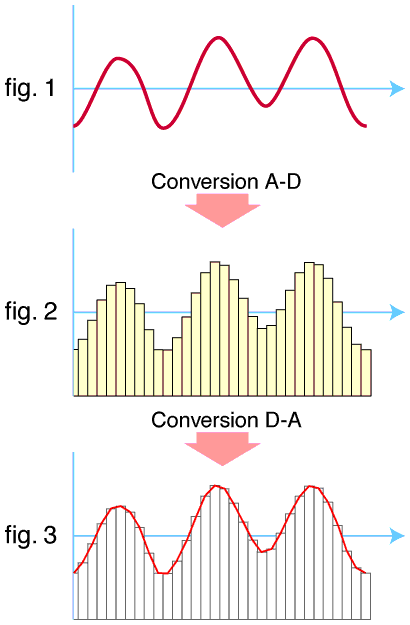
\includegraphics[width=0.6\textwidth]{Conversion_AD_DA.png}
    \caption{Procesul de conversie analog-digital și digital-analog\protect\footnotemark[1]}
    \label{fig:conversion-ad-da}
\end{figure}

\par
Acum că am definit cum sunt interpretate semnalele audio, putem să trecem la procesarea acestora.
Definim ce semnifică valorile obținute:

\begin{itemize}
    \item \textbf{Amplitudinea}: reprezintă presiunea undelor sonore măsurată la un moment de timp.
    Cu cât amplitudinea este mai mare, cu atât sunetul este mai puternic.
    \item \textbf{Ampitudinea zero}: valoarea 0 reprezintă linia de bază a semnalului audio, punctul
    principal de referință după care se măsoară amplitudinea.
    \item \textbf{Valori pozitive și negative}: valorile sunt reprezentate în formatul PCM (Pulse Code Modulation),
    unde valorile pozitive sunt reprezentate de valori între 0 și 1, iar valorile negative sunt reprezentate
    de valori între 0 și -1.
\end{itemize}
\footnotetext[1]{Imagine preluată de pe Wikipedia la adresa: \url{https://en.wikipedia.org/wiki/Analog-to-digital_converter}}

\begin{figure}[h]
    \centering
    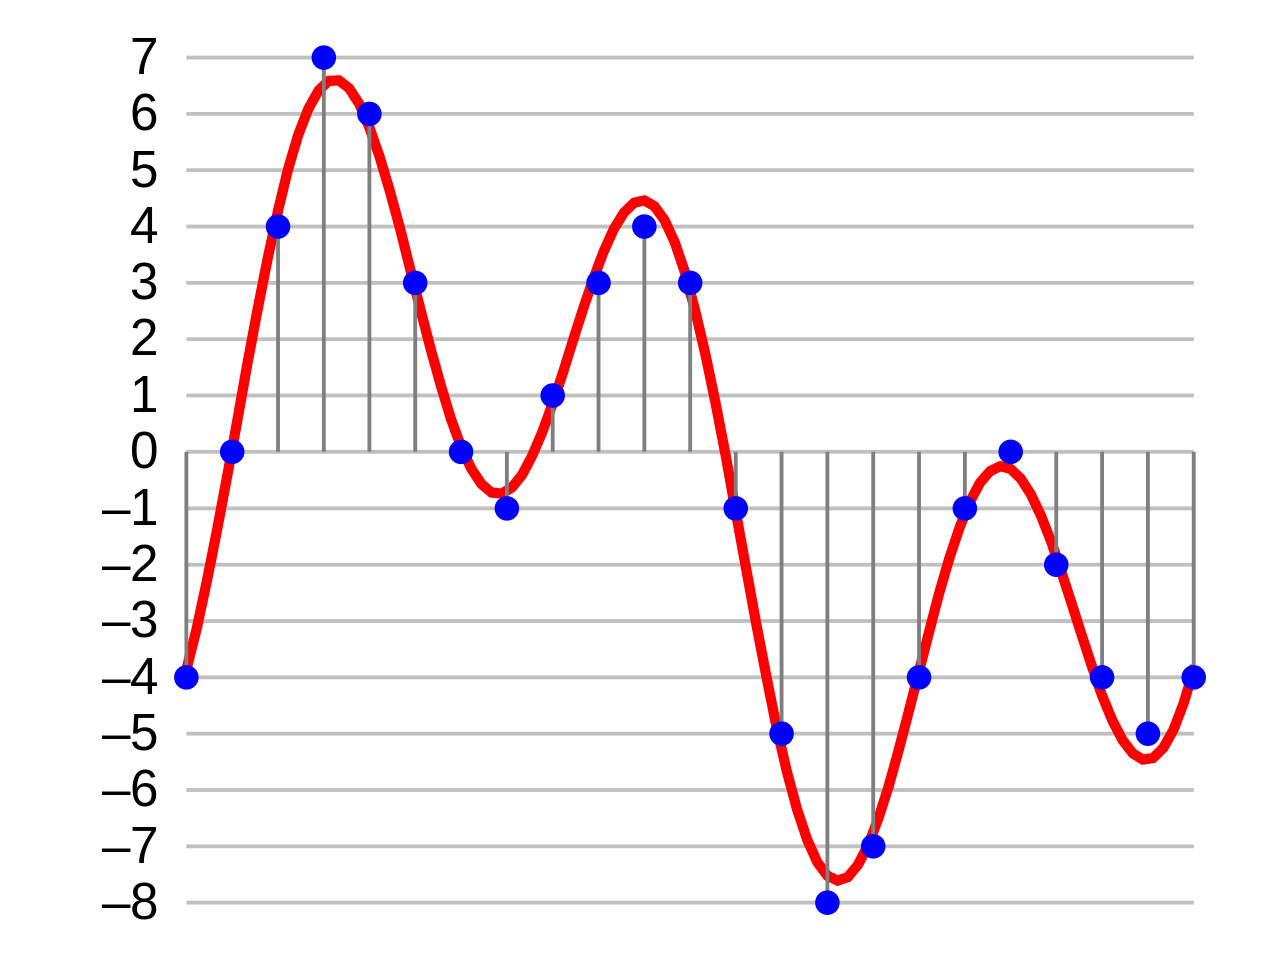
\includegraphics[width=0.5\textwidth]{PCM.png}
    \caption{Reprezentarea semnalului audio în format PCM\protect\footnotemark[2]}
    \label{fig:pcm}
\end{figure}

\par
De aici încolo vom lucra cu semnalul digital în Python folosind librăria \textit{soundfile},
\textit{librosa} și \textit{numpy} pentru a procesa secvențele audio.


\subsubsection{Controllers}
Pentru a menține logica din rute cât mai simplă, am creat un controller care se ocupă de procesarea
secvețelor audio primite de la serverul Express. 
\footnotetext[2]{Imagine preluată de pe Wikipedia la adresa: \url{https://en.wikipedia.org/wiki/Audio_bit_depth}}

\subsubsection{Procesarea secvențelor audio}
\par
Funcția \textbf{speech\_to\_text} primește ca parametru calea către fișierul audio salvat temporar,
îl deschide folosind \textit{soundfile} și îl transformă într-un șir de float-uri.
Sunt două tipuri de fișiere audio: \textbf{mono} și \textbf{stereo}, iar funcția trebuie să facă distincția
între cele două tipuri. 

\par
Formatul \textit{mono} are un singur canal audio, iar formatul \textit{stereo} are două canale audio, 
fiind conceput pentru a reda sunetul într-un mod mai realist. Deoarece modelul de recunoaștere a vorbirii
acceptă doar fișiere audio mono, am făcut media celor două canale pentru a obține un singur canal audio.

\par
De asemenea, modelul a fost antrenat pe fișiere audio cu o frecvență de eșantionare de 16kHz, așa că
în cazul în care frecvența fișierului audio este diferită (de exemplu, 44.1kHz), trebuie să o convertim
la 16kHz. Acest lucru se face folosind funcția \textit{resample} din librăria \textit{resampy}.

\par
Un aspect important, după cum am menționat și la seturile de date folosite, este că modelul a fost
antrenat pe fișiere audio cu o durată de aproximativ 10 secunde. O secvență audio prea mare oricum
nu ar încăpea în memoria serverului, așa că am ales să sparg secvența audio în segmente de câte 30 de
secunde folosind funcția \textit{stream} din librăria \textit{librosa}.

\par
Un alt aspect de luat în calcul aici, chiar dacă modelul ar putea procesa secvențe mai lungi, mai
intervine și timeout-ul socket-ului care ar putea expira în cazul unor secvențe prea mari. Deși în
cazul spargerii secvenței audio în segmente de câte 30 de secunde, se pot pierde informații de 
la începutul și finalul fiecărei bucăți, am ales să sacrific aceste informații pentru a asigura
procesarea cu succes a secvențelor audio. Exceptând aceste cazuri, bucățile pot fi tratate independent
și deci procesate în paralel, îmbunătățind semnificativ timpul de răspuns.

\subsubsection{Subtitrări}
\label{subsec:subtitles}
\par
Funcția \textbf{make\_subtitles} primește ca parametru textul transcris din fiecare block de 30 de secunde
și creează subtitrările în formatul .vtt. În cadrul unui bloc, modelul de recunoaștere a vorbirii 
folosește următoarele etape:
\begin{itemize}
    \item \textbf{Processing}: modelul primește secvența audio, și folosește procesorul specific de pe
    Hugging Face pentru a converti secvența audio în tensori. Vom numi acești tensori \textit{input\_values}.
    \item \textbf{Prediction}: modelul primește \textit{input\_values} și returnează \textit{logits}, tot
    sub forma de tensori reprezentând probabilitățile pentru fiecare literă din vocabular. Sunt calculate
    apoi \textit{predicted\_ids} fiind literele cu cele mai mari probabilități.
    \item \textbf{Decoding}: folosind \textit{logits}, modelul folosește algoritmul de decodare pentru a
    converti tensorii în text și obtinem \text{transcription}.
\end{itemize}

Astfel, obținem pentru fiecare bloc \textit{transcription}, \textit{input\_values} și \textit{predicted\_ids}.

\par
Pentru a crea subtitrările, folosim următoarele etape:

\begin{itemize}
    \item \textbf{ids\_w\_time}: cunoscând durata întregului bloc (30 de secunde) și numărul de token-uri
    prezis de model, putem estima momentul de timp al fiecărui token prin împărțirea indexului token-ului
    la numărul total de token-uri și înmulțirea cu durata blocului. Putem elimina token-urile pentru [PAD].
    \item \textbf{split\_ids\_w\_time}: folosind token-ul de delimitare între cuvinte, putem crea câte un 
    grup de token-uri între fiecare delimitator. Practic, obținem cuvintele propriu-zise, dar acum știm și
    momentul de timp.
    \item \textbf{word\_timestamps}: pentru fiecare cuvânt, calculăm momentul de timp de început și de sfârșit
    ca fiind minimul, respectiv maximul dintre toate momentele de timp ale token-urilor din acel cuvânt.
    \item \textbf{group\_timestamps}: putem grupa acum cuvintele în blocuri de 7 cuvinte, pentru a contura
    subtitrările. Începutul și sfârșitul fiecărui bloc de cuvinte este dat de momentul de timp al primului
    și ultimului cuvânt din bloc.
\end{itemize}

\begin{verbatim}
    
    predicted_ids: [6, 6, 0, 8, 0, 4, 4, 0, 17, 0, 5, 5, 0, 7, 0, 6,
                    \________/               \____________________/
                        to           |                meet
    0, 0, 4, 4, 0, 0, 18, 0, 0, 7, 0, 0, 12, 12, 4, 4, 6, 0, 0, 0, 8,
                       \_____________________/         \___________/
            |                    was              |          to           
    0, 4, 0, 0, 20, 0, 0, 10, 0, 0, 9, 0, 14, 0, 4, 4, 4, 5, 5, 7, 0,
                \_________________________/               \_________    
       |                   find                   |           each        
    19, 11, 0, 4, 4, 0, 0, 8, 8, 0, 6, 11, 11, 0, 5, 13, 0, 4, 4, 4]
    _____/                 \______________________/            |
                 |                   other

    words: ['to', 'meet', 'was', 'to', 'find', 'each', 'other']

    ids for letters and delimiter, but without pad

    [6, 6, 8, 4, 4, 17, 5, 5, 7, 6, 4, 4, 18, 7, 12, 12, 4, 4, 6, 8,
     \_____/        \____________/        \___________/        \__/
       to       |        meet         |        was        |     to
    4, 20, 10, 9, 14, 4, 4, 4, 5, 5, 7, 19, 11, 4, 4, 8, 8, 6, 11, 11,
    |  \___________/     |     \_____________/   |    \______________

    5, 13, 4, 4, 4]
    ____/     |

    split_ids_w_time

    'to' -> [(0.54, 6), (0.56, 6), (0.64, 8)]
    'meet' -> [(0.74, 17), (0.78, 5), (0.80, 5), (0.84, 7), (0.88, 6)]
    'was' -> [(1.48, 18), (1.54, 7), (1.60, 12), (1.62, 12)]
    'to' -> [(1.69, 6), (1.77, 8)]
    'find' -> [(1.87, 20), (2.01, 10), (2.07, 9), (2.11, 14)]
    'each' -> [(2.21, 5), (2.23, 5), (2.25, 7), (2.29, 19), (2.31, 11)]
    'other' -> [(2.43, 8), (2.45, 8), (2.49, 6), (2.51, 11), (2.53, 11),
                (2.57, 5), (2.59, 13)]

    word_timestamps

    'to' -> 0.54 - 0.64
    'meet' -> 0.74 - 0.88
    'was' -> 1.48 - 1.62
    'to' -> 1.69 - 1.77
    'find' -> 1.87 - 2.11
    'each' -> 2.21 - 2.31
    'other' -> 2.43 - 2.59

    group_timestamps

    'to meet was to find each other' -> 0.54 - 2.59
\end{verbatim}

\subsubsection{Formatarea subtitrărilor}
Funcția \textbf{save\_subtitles} primește ca parametru subtitrările și creează un fișier \textit{.vtt},
respectând formatul specificat. Fișierele în formatul \textit{.vtt} încep cu antetul \textit{WEBVTT},
iar pentru fiecare grup de subtitrări se specifică momentul de timp de început și de sfârșit, urmat
de textul subtitrării.
\par
Mai jos este un exemplu de subtitrare în formatul \textit{.vtt}:

\begin{verbatim}
    WEBVTT

    00:00:04.162 --> 00:00:06.424
    sometimes math and physics conspire in ways

    00:00:06.524 --> 00:00:07.665
    that just feel too good to be

    00:00:07.745 --> 00:00:09.706
    true let's play a strange sort of
\end{verbatim}


\par
Inspirat din issue-ul de pe GitHub: \url{https://github.com/huggingface/transformers/issues/11307}

\subsubsection{Config}
Configurările sunt folosite pentru a specifica serverului cum să proceseze cererile primite.
\begin{itemize}
    \item \textbf{ASR\_REPO}: numele modelului de recunoaștere a vorbirii folosit pentru a transcrie
    secvențele audio.
    \item \textbf{BOOSTED\_LM}: dacă este setat pe \textit{true}, folosește varianta îmbunătățită cu
    un n-gram language model pentru recunoașterea vorbirii.
    \item \textbf{SAMPLE\_RATE}: frecvența de eșantionare a fișierelor audio, setată pe 16kHz pentru
    a respecta cerințele modelului.
    \item \textbf{BLOCK\_SIZE}: lungimea blocurilor folosite în fluxul de date, setată pe 30 de secunde.
    \item \textbf{SPELL\_CHECK}: dacă este setat pe \textit{true}, folosește un model de corectare a
    cuvintelor pentru a îmbunătăți rezultatele.
\end{itemize}

\subsection{Flask Server - Clasificarea videoclip-urilor}
Serverul de Flask pentru clasificarea videoclip-urilor este similar cu cel pentru recunoașterea vorbirii,
dar are o structură mai simplă, nefiind necesare mai multe etape de procesare.
\subsubsection{Routes}
\par
Astfel, serverul definește o singură rută \textit{/topic} care primește cereri de tipul \textit{POST}
și returnează topicul textului primit. Deoarece secvența de intrare a modelului \textit{BERT} este 
limitată la 512 token-uri, am ales să împart textul în blocuri de câte 512 token-uri și fiecare bloc
este trimis la model pentru a obține topicul. Pentru a obține topicul final, se contorizează frecvența
apariției fiecărui topic și se returnează cel majoritar.
\subsubsection{Configurări}
\par
Serverul creează un \textit{pipeline} specific Hugging Face înaite de a primi cereri, pentru a reduce
timpul de răspuns. Acest \textit{pipeline} conține modelul preantrenat și fine-tunat pe setul de date
\textit{BBC News}. Mai multe detalii se regăsesc în secțiunea \ref{sec:clasificare-videoclipuri}.

\section{Baze de date}
Pentru stocarea datelor, am ales să folosesc două baze de date: MongoDB, datorită structurii sale
flexibile care permite dezvoltarea rapidă a aplicațiilor și Elasticsearch, pentru căutarea eficientă
în metadatele videoclip-urilor.
\subsection{MongoDB}
\subsubsection{Arhitectura bazei de date}
MongoDB este o bază de date de tip \textbf{NoSQL} care stochează datele sub forma de documente în 
formatul \textit{JSON}. Documentele sunt grupate în colecții, iar colecțiile sunt apoi grupate în
baze de date. 
\par
Intuitiv, un document este echivalentul unui rând dintr-o bază de date relațională, dar cu o structură
similară unui obiect JSON. Acesta permite stocarea datelor fără a respecta un model de date fix, adică
pot fi adăugate câmpuri noi, chiar și alte documente, diferite de celelalte documente din aceeași colecție.

\subsubsection{Structura datelor}

\par
Fiecare document conține, pe lângă datele propriu-zise, câmpuri speciale precum:
\begin{itemize}
    \item \textbf{\_id}: un \textit{ObjectId} adăugat automat de MongoDB pentru a identifica unic documentul.
    \item \textbf{\_v}: un câmp special care indică versiunea documentului în cazul actualizării. Acest
    câmp a fost conceput pentru a preveni conflictele de actualizare în cazul cererilor concurente.
    \item \textbf{createdAt} și \textbf{updatedAt}: câmpuri speciale de tipul \textit{ISODate} care
    indică momentul de creare și actualizare pentru fiecare document.
\end{itemize}

\subsubsection{Colecții}

\par
În cadrul aplicației noastre, am definit 3 colecții:
\begin{itemize}
    \item \textbf{users}: conține informații despre utilizatori precum: numele și prenumele, adresa de
    email, numele de utilizator, parola criptată și url-ul către poza de profil.
    \item \textbf{videos}: conține informații despre videoclipuri precum: titlul, descrierea, topicul,
    id-ul autorului (referință către colecția \textit{users}), url-ul către videoclip, url-ul către
    subtitrări și două liste separate pentru id-urile utilizatorilor care au dat like și dislike.
    \item \textbf{comments}: conține informații despre comentarii precum: textul comentariului, 
    id-ul autorului (referință către colecția \textit{users}), id-ul videoclipului (referință către
    colecția \textit{videos}), isDeleted folosit la \textit{soft-delete} și \textit{hard-delete}, 
    parentId în cazul în care comentariul este un răspuns la alt comentariu.
\end{itemize}

\subsubsection{Interacțiunea cu baza de date}

\par
Interacțiunea cu baza de date are loc cu ajutorul librăriei \textit{mongoose} care definește modelele
în serverul Express și execută operații de tip CRUD (Create, Read, Update, Delete) în baza de date.
\textit{mongoose} este un ODM (Object Data Modeling) care oferă un nivel de abstractizare peste MongoDB
și permite definirea de scheme pentru documente, validarea datelor și crearea de relații între colecții.

\par
Un alt aspect important pus la dispoziție de \textbf{MongoDB} îl reprezintă capacitatea de a crea replici
la nivel de colecție, numite \textit{indexes}. Deși aplicația noastră este un prototip, nu are nevoie 
de scalările orizontale, dar în cazul unui volum mare de date, replicile facilitează operațiile de
citire și scriere, îmbunătățind timpul de răspuns.

\subsection{Cron Jobs}
\label{sec:cron-jobs}
\subsubsection{Definiție și utilitate}
Un \textbf{cron job} este un proces care rulează automat la un momente de tip prestabilite. În cadrul proiectului,
un \textit{cron job} își găsește utilitatea în procesul de curățare al arborelui de comentarii pentru fiecare 
videoclip. Problema constă în găsirea unei soluții eficiente care șterge comentariile marcate drept \textit{soft-delete}
cu subarborele de răspunsuri gol.
\par
Figura de mai jos ilustrează acest concept:
\begin{verbatim}
    Cool video!
    |__ Indeed it is!
    |__ |__ [deleted] (1)
    |__ [deleted] (2)
    |__ |__ Waiting for the next one!
    [deleted] (3)
    Awesome!
    |__ [deleted] (4)
    |__ |__ Yeah, I agree!
    |__ [deleted] (5)
    |__ |__ [deleted] (6)
\end{verbatim}

\par
În exemplul de mai sus, comentariile cu textul [deleted] sunt marcate drept \textit{soft-delete}, semnificând că
deși au fost șterse de utilizator, ele încă există în baza de date. 
\par
Problema apare atunci când un comentariu este marcat drept \textit{soft-delete}, dar nu știm, fără o parcurege în 
prealabil, dacă poate fi șters sau nu.


\par
O primă idee ar fi ca de fiecare dată când un comentariu este șters, să facem o cerere pentru întreg arborele
de comentarii și să verificăm dacă fiecare nod are copii care pot fi la rândul lor șterși. Această metodă
este ineficientă, deoarece necesită o cantitate mare de resurse pentru a parcurge întreg arborele de comentarii
la fiecare actualizare.

\par
O altă soluție ar fi să păstrăm comentariile în starea \textit{soft-delete} și să rulăm un \textit{cron job}
la intervale regulate de timp care să curețe arborele de comentarii. 

\subsubsection{Algoritm}
\par
Algoritmul de curățare a arborelui de comentarii este următorul:

\begin{itemize}
    \item \textbf{Inițializare}: creează conexiunea cu baza de date, obține toate comentariile și creează
    structura arborescentă menționată anterior.
    \item \textbf{Parcurgere}: parcurge arborele în adâncime folosind algoritmul DFS (Depth First Search) și
    verifică recursiv folosind conceptul de programare dinamică, dacă un nod poate fi șters sau nu. La fiecare
    pas din recursie se verifică dacă nodul curent este marcat drept \textit{soft-delete} și dacă toți
    subarborii copiilor săi sunt de asemenea marcați drept \textit{soft-delete}. În caz afirmativ, nodul
    curent poate fi șters și este adăugat într-o listă de noduri \textit{deletable}. Altfel, nodul nu poate
    fi șters și implicit toate nodurile de pe drumul până la rădăcină nu pot fi șterse.
    \item \textbf{Ștergere}: după ce arborele a fost parcurs și a fost creată lista \textit{deletable}, se
    apelează iar clientul MongoDB pentru a șterge toate nodurile din listă.
\end{itemize}

\par
Exemplul de mai jos ilustrează algoritmul de curățare a arborelui de comentarii:

\vspace{2em}

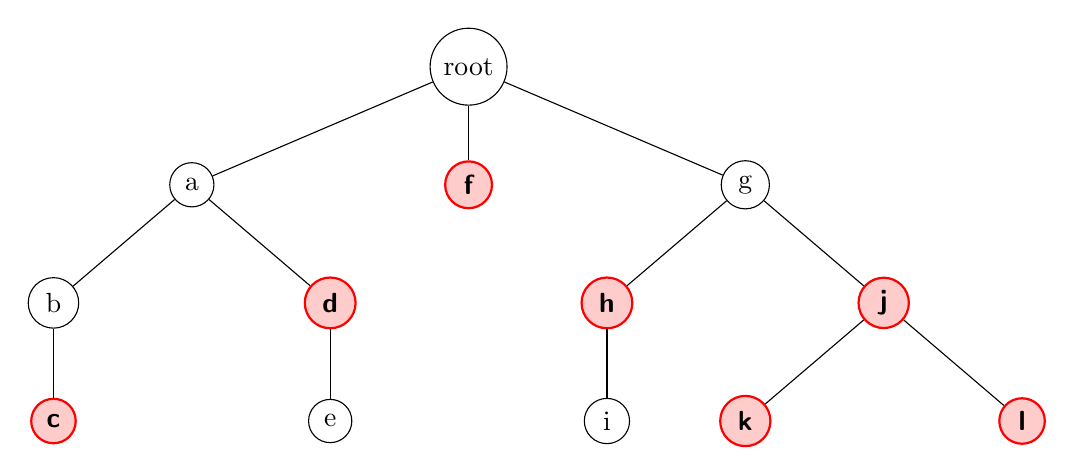
\begin{tikzpicture}[sibling distance=10em, every
    node/.style = {shape=circle, draw, align=center},
    highlightSoftDelete/.style = {fill=red!20, draw=red, thick, font=\sffamily\bfseries},
    ]
    \node {root}
      child { node {a}
        child { node {b} 
          child { node [highlightSoftDelete] {c} } }
        child { node [highlightSoftDelete] {d}
          child { node {e} } } }
      child { node [highlightSoftDelete] {f} }
      child { node {g}
        child { node [highlightSoftDelete] {h}
          child { node {i} } }
        child { node [highlightSoftDelete] {j}
          child { node [highlightSoftDelete] {k} } 
          child { node [highlightSoftDelete] {l} } 
          } };
\end{tikzpicture}

\vspace{2em}

\par
În arborele prezentat, nodurile colorate cu roșu reprezintă comentariile \textit{soft-delete}. Algoritmul
va adăuga nodurile \textit{c}, \textit{f}, \textit{j}, \textit{k} și \textit{l} în lista \textit{deletable}.
\par
Chiar dacă nodurile \textit{d} și \textit{h} sunt marcate drept \textit{soft-delete}, ele nu pot fi șterse
permanent (\textit{hard-delete}) din cauza subarborilor încă activi.

\subsection{Elasticsearch}
\subsubsection{Concept}
Elasticsearch este un motor de căutare ce organizează datele în documente în formatul \textit{JSON} care
sunt apoi grupate în indici. Indicii sunt echivalentul bazelor de date din MongoDB, iar documentele sunt
echivalentul rândurilor din tabelele relaționale.

\par
Concepte cheie în Elasticsearch:
\begin{itemize}
    \item \textbf{Document}: unitatea de bază folosită de Elasticsearch în formatul \textit{JSON}
    (considerat formatul standard pentru transferul de date)
    \item \textbf{Indices}: o colecție de documente cu trăsături similare formează un indice și reprezintă
    cel mai înalt nivel de organizare a datelor.
    \item \textbf{Inverted Index}: reprezintă mecanismul care stă la baza motoarelor de căutare și constă
    într-o structură de date (similară cu un hashmap) care mapează cuvintele (sau mai bine zis, termenii)
    la locațiile unde apar în documente. Astfel, fiecare document este împărțit în termeni individuali 
    care sunt folosiți la căutare.
\end{itemize}

\par
Figura \ref{fig:elasticsearch} ilustrează conceptul \textit{Inverted Index}. \cite{elasticsearchexplained}

\subsubsection{Inserare}
\par
În cazul aplicației noastre, am definit un singur indice \textit{videos} care conține metadatele
videoclip-urilor: titlul, descrierea, topicul și subtitrările. De fiecare dată când un videoclip
este încărcat în aplicație, inserarea se face atât în baza de date MongoDB, cât și în Elasticsearch.

\begin{figure}[h]
    \centering
    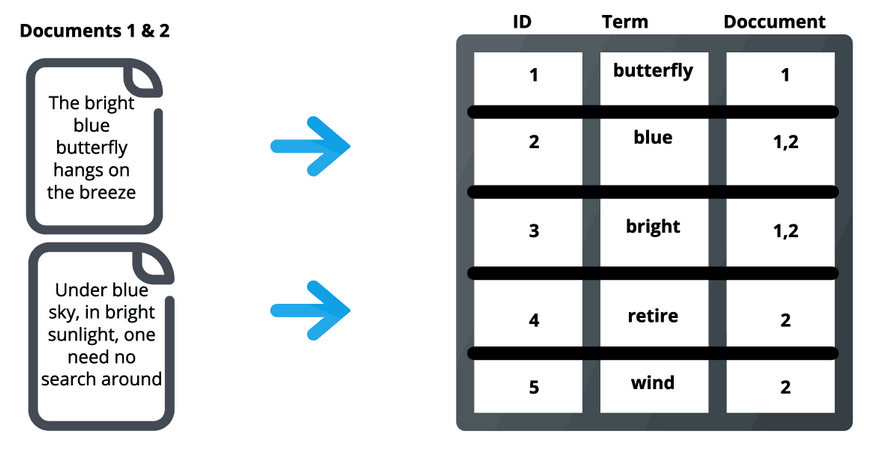
\includegraphics[width=0.6\textwidth]{elasticsearch.png}
    \caption{Inverted Index\protect\footnotemark[3]}
    \label{fig:elasticsearch}
\end{figure}

\footnotetext[3]{Imagine preluată de pe site-ul knowi.io la adresa: \url{https://www.knowi.com/blog/what-is-elastic-search/}}

\subsubsection{Căutare}
Interogarea în Elasticsearch permite specificarea criteriului de căutare precum: full-text, fuzzy, prefix,
expresii regulate etc. În cazul aplicației noastre, am ales să folosesc \textit{fuzziness AUTO} pentru a 
permite căutarea cuvintelor similare cu cele din cerere.

\section{Deployment}
\subsection{Docker}

\subsubsection{Concept}
Docker este o platformă care permite dezvoltatorilor să izoleze logica, dependințele și mediul de lucru
în containere. Spre deosebire de mașinile virtuale, Docker nu virtualizează întregul sistem de operare,
ci combină aplicația și dependințele sale cu librăriile oferite de sistemul de operare.
\par
În contextul mașinilor virtuale (VM), alocarea de resurse este dirijată de un \textit{hypervisor} care
gestionează resursele fizice ale sistemului. În mod asemănător, Docker folosește un sistem de gestiune
al resurselor mult mai eficient din punct de vedere al memoriei și timpului de rulare. 
\par
Avantajele folosirii containerelor Docker sunt:
\begin{itemize}
    \item \textbf{memorie mică}: un container Docker nu conține întregul sistem de operare, ci doar
    procesele și dependințele necesare pentru aplicație, dimensiunea acestuia fiind de ordinul MB.
    \item \textbf{portabilitate}: rezolvă problema \textit{it works on my machine} datorită
    izolării mediului de lucru cu ajutorul imaginilor și containerelor.
    \item \textbf{utilizare eficientă a resurselor}: permite gestionarea eficientă a resurselor sistemului.
\end{itemize}

\subsubsection{Dockerfile și Docker image}
\par
Imaginile Docker reprezintă unitatea de bază a containerelor și conțin tot ce este necesar (codul sursă,
dependințele, tool-urile, librăriile, variabile de mediu etc.) pentru a rula o aplicație. Imaginile
sunt structurate în nivele de abstractizare construite pe baza unui fișier numit \textit{Dockerfile}.
\par
Un \textit{Dockerfile} enumeră instrucțiunile necesare pentru construirea imaginii. De obicei, se pleacă
de la o imagine de bază (de exemplu, \textit{python:3.8-slim}), după care se instalează dependințele
necesare și se copiază codul sursă în container. În ultima parte a fișierului, se specifică comanda
care pornește aplicația.
\par
Odată ce \textit{Dockerfile}-ul este definit, se pot construi imagini Docker folosind comanda \textit{docker build},
eventual cu argumente suplimentare în linia de comandă. (de exemplu, menționarea portului pe care rulează aplicația, 
versiunea imaginii etc.)

\subsubsection{Docker container}
\par
Un container de Docker folosește imaginea construită anterior și creează instanțe ale acesteia. În timp ce
o imagine permite doar citirea, un container permite dezvoltatorului interacțiunea cu acesta, fie pentru
a rula comenzi, fie pentru a monitoriza starea aplicației.

\begin{figure}[h]
    \centering
    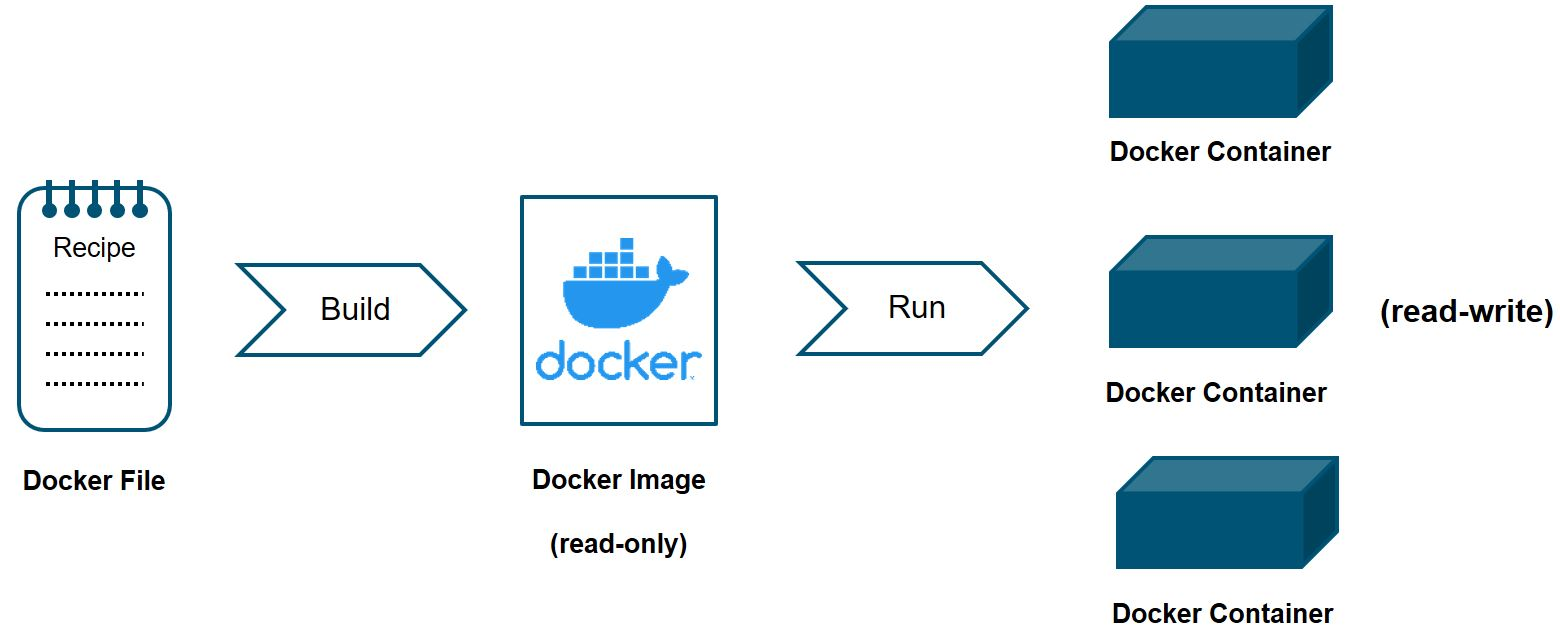
\includegraphics[width=0.6\textwidth]{docker.JPG}
    \caption{Docker\protect\footnotemark[4]}
    \label{fig:docker}
\end{figure}
\footnotetext[4]{Imagine preluată de pe site-ul suresoft la adresa: \url{https://suresoft.gitlab-pages.rz.tu-bs.de/workshop-website/continuous-integration/containers.html}}

\subsubsection{Docker Compose}
\par
Pe parcursul dezvoltării aplicației, apar din ce în ce mai multe servicii care trebuie gestionate separat
și care depind unele de altele. Docker Compose este un tool care înglobează toate comenzile necesare
pentru pornirea și oprirea serviciilor, precum și pentru construirea imaginilor și a containerelor.
\par
Docker Compose folosește un fișier numit \textit{docker-compose.yml} care conține toate detaliile necesare
pentru fiecare serviciu, dintre care amintim: imaginea folosită, numele containerului, porturile expuse,
variabilele de mediu, volumele, dependințele între alte servicii, rețelele folosite etc.

\subsubsection{Volume și rețele}
\par
În cazul în care aplicația are nevoie de o stocare persistentă, de pildă pentru bazele de date, se pot
folosi volume Docker. Un volum Docker este, de fapt, un director din sistemul gazdă care este montat în
container al cărui conținut este persistent chiar și după oprirea containerului.

\par
De asemenea, Docker oferă și posibilitatea de a crea rețele virtuale prin intermediul cărora serviciile
pot comunica între ele. Implicit, Docker oricum atribuia fiecărui container o adresă IP, dar în cazul
pornirilor succesive ale aceluiași container, adresa IP se schimbă și nu mai poate fi accesată. Folosirea
rețelelor Docker permite atribuirea manuală a IP-urilor.

\subsection{Dockerizarea aplicației}
\par
Aplicația beneficiază de avantajele oferite de Docker și Docker Compose pentru a simplifica procesul
de dezvoltare și de deployment. În cadrul proiectului, am definit următoarele servicii:

\begin{itemize}
    \item \textbf{MongoDB Container}: rulează o instanță de MongoDB pentru stocarea datelor, folosind
    un volum Docker pentru a asigura persistența datelor și făcând o corespondență între portul gazdă
    și portul containerului.
    \item \textbf{Elasticsearch Container}: rulează o instanță de Elasticsearch pentru căutarea eficientă
    în metadatele videoclip-urilor, folosind de asemenea un volum Docker.
    \item \textbf{Flask Server - Recunoașterea Vorbirii}: rulează serverul Flask pentru recunoașterea
    vorbirii, folosind portul 5001. Deoarece serverul comunică cu MongoDB și Elasticsearch, cele două
    servicii sunt specificate ca dependințe.
    \item \textbf{Flask Server - Clasificarea Videoclipurilor}: rulează serverul Flask pentru clasificarea
    videoclipurilor, folosind portul 5003. Nu are dependințe.
\end{itemize}

\par
Pentru serverele de React si Node.js am ales să nu folosesc containere Docker astfel încât să pot
beneficia de o dezvoltarea rapidă și de actualizare în timp real a codului sursă.

